\documentclass[12pt]{llncs}
%\documentclass{jktr}

\usepackage[pdftex]{hyperref}                   
\usepackage {mathpartir}
\usepackage{bigpage}
\usepackage{bcprules}
\usepackage {listings}
\usepackage{amsmath}
\usepackage{amssymb}
\usepackage{amsfonts}
\usepackage{amstext}
\usepackage{latexsym}
\usepackage{longtable}
\usepackage{stmaryrd}
\usepackage{graphicx} 
%\usepackage[margins=2.5cm,nohead,nofoot]{geometry}
%\usepackage{geometry}
\usepackage{color}
\usepackage{xcolor}

\graphicspath{ {.} }


%\include{myPreamble}

% Double brackets
\newcommand{\ldb}{[\![}
\newcommand{\rdb}{]\!]}
\newcommand{\ldrb}{(\!(}
\newcommand{\rdrb}{)\!)}
\newcommand{\lrbb}{(\!|}
\newcommand{\rrbb}{|\!)}
\newcommand{\lliftb}{\langle\!|}
\newcommand{\rliftb}{|\!\rangle}
%\newcommand{\plogp}{:\!-}
\newcommand{\plogp}{\leftarrow}
%\newcommand{\plogp}{\coloneq}
% \newcommand{\lpquote}{\langle}
% \newcommand{\rpquote}{\rangle}
% \newcommand{\lpquote}{\lceil}
% \newcommand{\rpquote}{\rceil}
\newcommand{\lpquote}{\ulcorner}
\newcommand{\rpquote}{\urcorner}
\newcommand{\newkw}{\nu}
\newcommand{\dblhdlarrow}{\texttt{<\!<\!-}}
\newcommand{\dbltllarrow}{\texttt{<\!=}}
\newcommand{\sngllarrow}{\texttt{<\!-}}
\newcommand{\dblhdlrarrow}{\texttt{<\!<\!-\!>\!>}}
\newcommand{\dbltllrarrow}{\texttt{<\!=\!>}}
\newcommand{\sngllrarrow}{\texttt{<\!-\!>}}

% SYNTAX
\newcommand{\id}[1]{\texttt{#1}}
\newcommand{\none}{\emptyset}
\newcommand{\eps}{\epsilon}
\newcommand{\set}[1]{\{#1\}}
\newcommand{\rep}[2]{\id{\{$#1$,$#2$\}}}
\newcommand{\elt}[2]{\id{$#1$[$#2$]}}
\newcommand{\infinity}{$\infty$}

\newcommand{\pzero}{\mathsf{0}}
\newcommand{\seq}{\mathsf{\id{,}}}
\newcommand{\all}{\mathsf{\id{\&}}}
\newcommand{\choice}{\mathsf{\id{|}}}
\newcommand{\altern}{\mathsf{\id{+}}}
\newcommand{\juxtap}{\mathsf{\id{|}}}
\newcommand{\concat}{\mathsf{.}}
\newcommand{\punify}{\mathsf{\id{:=:}}}
\newcommand{\fuse}{\mathsf{\id{=}}}
\newcommand{\scong}{\mathsf{\equiv}}
\newcommand{\nameeq}{\mathsf{\equiv_N}}
\newcommand{\alphaeq}{\mathsf{\equiv_{\alpha}}}
\newcommand{\arrvec}[1]{\overrightarrow{#1}}
\newcommand{\names}[1]{\mathsf{N}(#1)}
\newcommand{\freenames}[1]{\mathsf{FN}(#1)}
\newcommand{\boundnames}[1]{\mathsf{BN}(#1)}
%\newcommand{\lift}[2]{\texttt{lift} \; #1 \concat #2}
\newcommand{\binpar}[2]{#1 \mathsf{|} #2}
\newcommand{\outputp}[2]{#1\mathsf{!}(#2)}
\newcommand{\prefix}[3]{\mathsf{for(}#2 \leftarrow #1 \mathsf{)} #3}
%%\newcommand{\lift}[2]{#1 \lliftb #2 \rliftb}
\newcommand{\lift}[2]{#1 \mathsf{!}(#2)}
\newcommand{\clift}[1]{\lliftb #1 \rliftb}
\newcommand{\quotep}[1]{\mathsf{@} #1}
\newcommand{\dropn}[1]{\mathsf{*} #1}
\newcommand{\procn}[1]{\stackrel{\cdot}{#1}}
\newcommand{\spacen}[2]{\mathsf{@}\langle #1, #2 \rangle}

\newcommand{\newp}[2]{(\newkw \; #1 ) #2}
\newcommand{\bangp}[1]{! #1}

\newcommand{\substp}[2]{\{ \quotep{#1} / \quotep{#2} \}}
\newcommand{\substn}[2]{\{ #1 / #2 \}}

\newcommand{\psubstp}[2]{\widehat{\substp{#1}{#2}}}
\newcommand{\psubstn}[2]{\widehat{\substn{#1}{#2}}}

\newcommand{\applyp}[2]{#1 \langle #2 \rangle}
\newcommand{\absp}[2]{( #1 ) #2}
\newcommand{\annihilate}[1]{#1^{\times}}
\newcommand{\dualize}[1]{#1^{\bullet}}
\newcommand{\ketp}[1]{\mathsf{|}#1 \rangle}
\newcommand{\brap}[1]{\langle #1 \mathsf{|}}
\newcommand{\testp}[2]{\langle #1 \mathsf{|} #2 \rangle}
\newcommand{\testnp}[3]{\langle #1 \mathsf{|} #2 \mathsf{|} #3 \rangle}

\newcommand{\transitions}[3]{\mathbin{#1 \stackrel{#2}{\longrightarrow} #3}}
\newcommand{\meaningof}[1]{\ldb #1 \rdb}
\newcommand{\pmeaningof}[1]{\ldb #1 \rdb}
\newcommand{\nmeaningof}[1]{\lrbb #1 \rrbb}

\newcommand{\Proc}{\mathsf{Proc}}
\newcommand{\QProc}{\quotep{\mathsf{Proc}}}
\newcommand{\MixSumProc}{\mathsf{MixSumProc}}

\newcommand{\entailm}{\mathbin{\vdash_{\mathfrak m}}} %matching
\newcommand{\entailp}{\mathbin{\vdash_{\mathfrak p}}} %behavioral
\newcommand{\entailv}{\mathbin{\vdash_{\mathfrak v}}} %validation
\newcommand{\congd}{\mathbin{\equiv_{\mathfrak d}}}
\newcommand{\congs}{\mathbin{\equiv_{\mathfrak s}}}
\newcommand{\congp}{\mathbin{\equiv_{\mathfrak p}}}
%\newcommand{\logequiv}{\mathbin{\leftrightarrow}}

\newcommand{\barb}[2]{\mathbin{#1 \downarrow_{#2}}}
\newcommand{\dbarb}[2]{\mathbin{#1 \Downarrow_{#2}}}

% From pi-duce paper
\newcommand{\red}{\rightarrow}
\newcommand{\wred}{\Rightarrow}
\newcommand{\redhat}{\hat{\longrightarrow}}
\newcommand{\lred}[1]{\stackrel{#1}{\longrightarrow}} %transitions
\newcommand{\wlred}[1]{\stackrel{#1}{\Longrightarrow}}

\newcommand{\opm}[2]{\overline{#1} [ #2 ]} % monadic
\newcommand{\ipm}[2]{{#1} ( #2 )} 
\newcommand{\ipmv}[2]{{#1} ( #2 )} % monadic
\newcommand{\parop}{\;|\;}		% parallel operator
\newcommand{\patmatch}[3]{#2 \in #3 \Rightarrow #1}
\newcommand{\sdot}{\, . \,}		% Space around '.'
\newcommand{\bang}{!\,}
%\newcommand{\fuse}[1]{\langle #1 \rangle}		
\newcommand{\fusion}[2]{#1 = #2} % fusion prefix/action
\newcommand{\rec}[2]{\mbox{\textsf{rec}} \, #1. \, #2}
\newcommand{\match}[2]{\mbox{\textsf{match}} \; #1 \; \mbox{\textsf{with}} \; #2}
\newcommand{\sep}{:}
\newcommand{\val}[2]{\mbox{\textsf{val}} \; #1 \; \mbox{\textsf{as}} \; #2}

\newcommand{\rel}[1]{\;{\mathcal #1}\;} %relation
\newcommand{\bisim}{\stackrel{.}{\sim}_b} %bisimilar
\newcommand{\wb}{\approx_b} %weak bisimilar
\newcommand{\bbisim}{\stackrel{\centerdot}{\sim}} %barbed bisimilar
\newcommand{\wbbisim}{\stackrel{\centerdot}{\approx}} %weak barbed bisimilar
\newcommand{\bxless}{\lesssim}	%expansion less (amssymb required)
\newcommand{\bxgtr}{\gtrsim}	%expansion greater (amssymb required)
\newcommand{\beq}{\sim}		%barbed congruent
\newcommand{\fwbeq}{\stackrel{\circ}{\approx}}	%weak barbed congruent
\newcommand{\wbeq}{\approx}	%weak barbed congruent
\newcommand{\sheq}{\simeq}	%symbolic hypereq
\newcommand{\wbc}{\approx_{cb}}

% rho logic

\newcommand{\ptrue}{\mathbin{true}}
\newcommand{\psatisfies}[2]{#1 \models #2}
\newcommand{\pdropf}[1]{\rpquote #1 \lpquote}
\newcommand{\plift}[2]{#1 \lliftb #2 \rliftb}
\newcommand{\pprefix}[3]{\langle #1 ? #2 \rangle #3}
\newcommand{\pgfp}[2]{\textsf{rec} \; #1 \mathbin{.} #2}
\newcommand{\pquant}[3]{\forall #1 \mathbin{:} #2 \mathbin{.} #3}
\newcommand{\pquantuntyped}[2]{\forall #1 \mathbin{.} #2}
\newcommand{\riff}{\Leftrightarrow}

\newcommand{\PFormula}{\mathbin{PForm}}
\newcommand{\QFormula}{\mathbin{QForm}}
\newcommand{\PropVar}{\mathbin{\mathcal{V}}}

% qm notation
\newcommand{\state}[1]{\juxtap #1 \rangle}
\newcommand{\event}[1]{\langle #1 \juxtap}
\newcommand{\innerprod}[2]{\langle #1 \juxtap #2 \rangle}
\newcommand{\prmatrix}[2]{\juxtap #1 \rangle \langle #2 \juxtap}
\newcommand{\fprmatrix}[3]{\juxtap #1 \rangle #2 \langle #3 \juxtap}

% End piduce contribution

\newcommand{\typedby}{\mathbin{\:\colon}}
\newcommand{\mixedgroup}[1]{\id{mixed($#1$)}}
\newcommand{\cast}[2]{\id{CAST AS} \; #1 \; (#2)}
\newcommand{\bslsh}{\mathbin{\id{\\}}}
\newcommand{\bslshslsh}{\mathbin{\id{\\\\}}}
\newcommand{\fslsh}{\mathbin{\id{/}}}
\newcommand{\fslshslsh}{\mathbin{\id{//}}}
\newcommand{\bb}[1]{\mbox{#1}}
\newcommand{\bc}{\mathbin{\mathbf{::=}}}
\newcommand{\bm}{\mathbin{\mathbf\mid}}
%\newcommand{\bm}{\mathbin{\mathbf\mid}}
\newcommand{\be}{\mathbin{=}}
\newcommand{\bd}{\mathbin{\buildrel {\rm \scriptscriptstyle def} \over \be}}
%\newcommand{\category}[1]{\mbox{\bf #1}}

\newcommand{\prefixt}[3]{\mathbf{for}\mathbf{(}\mathbf{#2} \leftarrow \mathbf{#1} \mathbf{)} \mathbf{#3}}
\newcommand{\outputt}[2]{\mathbf{#1}\mathsf{!}(\mathbf{#2})}
\newcommand{\dropt}[1]{\mathbf{*} \mathbf{#1}}
\newcommand{\quotet}[1]{\mathbf{@} \mathbf{#1}}
\newcommand{\commr}[4]{\mathsf{comm(}#1, #2, #3, #4  \mathsf{)}}
\newcommand{\commt}[4]{\mathbf{comm(}\mathbf{#1}, \mathbf{#2}, \mathbf{#3}, \mathbf{#4} \mathbf{)}}
\newcommand{\binparx}[2]{\mathsf{par}(#1, #2)}
\newcommand{\binpart}[2]{\mathbf{par}(\mathbf{#1}, \mathbf{#2})}
\newcommand{\binparpt}[2]{\mathbf{#1} \mathbf{\mathsf{|}} \mathbf{#2}}
\newcommand{\binpartl}[2]{\mathbf{par}_{L}(\mathbf{#1}, \mathbf{#2})}
\newcommand{\binpartr}[2]{\mathbf{par}_{R}(\mathbf{#1}, \mathbf{#2})}

%GRAMMAR
\newlength{\ltext}
\newlength{\lmath}
\newlength{\cmath}
\newlength{\rmath}
\newlength{\rtext}

\settowidth{\ltext}{complex type name}
\settowidth{\lmath}{$xxx$}
\settowidth{\cmath}{$::=$}
\settowidth{\rmath}{\id{attributeGroup}}
\settowidth{\rtext}{repetition of $g$ between $m$ and $n$ times}

\newenvironment{grammar}{
  \[
  \begin{array}{l@{\quad}rcl@{\quad}l}
  \hspace{\ltext} & \hspace{\lmath} & \hspace{\cmath} & \hspace{\rmath} & \hspace{\rtext} \\
}{
  \end{array}\]
}

% Over-full v-boxes on even pages are due to the \v{c} in author's name
%\vfuzz2pt % Don't report over-full v-boxes if over-edge is small

% THEOREM Environments ---------------------------------------------------
% MATH -------------------------------------------------------------------
 \newcommand{\veps}{\varepsilon}
 \newcommand{\To}{\longrightarrow}
 \newcommand{\h}{\mathcal{H}}
 \newcommand{\s}{\mathcal{S}}
 \newcommand{\A}{\mathcal{A}}
 \newcommand{\J}{\mathcal{J}}
 \newcommand{\M}{\mathcal{M}}
 \newcommand{\W}{\mathcal{W}}
 \newcommand{\X}{\mathcal{X}}
 \newcommand{\BOP}{\mathbf{B}}
 \newcommand{\BH}{\mathbf{B}(\mathcal{H})}
 \newcommand{\KH}{\mathcal{K}(\mathcal{H})}
 \newcommand{\Real}{\mathbb{R}}
 \newcommand{\Complex}{\mathbb{C}}
 \newcommand{\Field}{\mathbb{F}}
 \newcommand{\RPlus}{\Real^{+}}
 \newcommand{\Polar}{\mathcal{P}_{\s}}
 \newcommand{\Poly}{\mathcal{P}(E)}
 \newcommand{\EssD}{\mathcal{D}}
 \newcommand{\Lom}{\mathcal{L}}
 \newcommand{\States}{\mathcal{T}}
 \newcommand{\abs}[1]{\left\vert#1\right\vert}
% \newcommand{\set}[1]{\left\{#1\right\}}
%\newcommand{\seq}[1]{\left<#1\right>}
 \newcommand{\norm}[1]{\left\Vert#1\right\Vert}
 \newcommand{\essnorm}[1]{\norm{#1}_{\ess}}

%%% NAMES
\newcommand{\Names}{{\mathcal N}}
\newcommand{\Channels}{{\sf X}}
\newcommand{\Variables}{{\mathcal V}}
\newcommand{\Enames}{{\mathcal E}}
\newcommand{\Nonterminals}{{\mathcal S}}
\newcommand{\Pnames}{{\mathcal P}}
\newcommand{\Dnames}{{\mathcal D}}
\newcommand{\Types}{{\mathcal T}}

\newcommand{\fcalc}{fusion calculus}
\newcommand{\xcalc}{${\mathfrak x}$-calculus}
\newcommand{\lcalc}{$\lambda$-calculus}
\newcommand{\pic}{$\pi$-calculus}
\newcommand{\spic}{spi-calculus}
\newcommand{\rhoc}{$\rho$-calculus}
\newcommand{\rhol}{$\rho$-logic}
\newcommand{\hcalc}{highwire calculus}
\newcommand{\dcalc}{data calculus}
%XML should be all caps, not small caps. --cb
%\newcommand{\xml}{\textsc{xml}}
\newcommand{\xml}{XML} 
 

%\ifpdf
%\usepackage[pdftex]{graphicx}
%\else
%\usepackage{graphicx}
%\fi

 % \ifpdf
%  \usepackage{pdfsync}
%  \if


%\title{Brief Article}
%\author{David F. Snyder}
%\author{L.G. Meredith}

%\address{Dept. of Math., Texas State University--San Marcos, San Marcos, TX 78666}
       
\pagestyle{empty}


\begin{document}

\lstset{language=[Objective]Caml,frame=shadowbox}

\def\lastname{Meredith}

\title{The MeTTa calculus}
\titlerunning{rho20}

\author{ L.G. Meredith\inst{1} }
\institute{ CEO, F1R3FLY.io 9336 California Ave SW, Seattle, WA 98103, USA, \\
  \email{ ceo@f1r3fly.io } 
} 

\maketitle              % typeset the title of the contribution

%%% ----------------------------------------------------------------------

\begin{abstract}

  We describe a core calculus that captures the operational semantics
  of the language $\mathsf{MeTTa}$.

\end{abstract}

%\keywords{Process calculi, knots, invariants}

% \begin{keyword}
% concurrency, message-passing, process calculus, reflection, program logic
% \end{keyword}

%\end{frontmatter}


\section{Introduction and motivation}

In \cite{arxiv:meta-metta-opsem:meredith} we described a register
machine based operational semantics for $\mathsf{MeTTa}$. While this
has some utility for proving the correctness of compilers, it is not
conducive for reasoning about types and other more abstract aspects of
$\mathsf{MeTTa}$-based computation. Here we present a calculus,
together with an efficient implementation and prove the correctness of
the implementation.

Additionally, we use the $\mathsf{OSLF}$ algorithm developed by
Meredith, Stay, and Williams to calculate a spatial-behavioral type
system for $\mathsf{MeTTa}$. Further, we adapt a well known procedure
for proving the termination of rewrites to provide a token-based
security model for the calculus and implementation. Beyond that we
derive versions of fuzzy, stochastic, and quantum execution modes,
automatically.

\begin{figure}
  \centering
  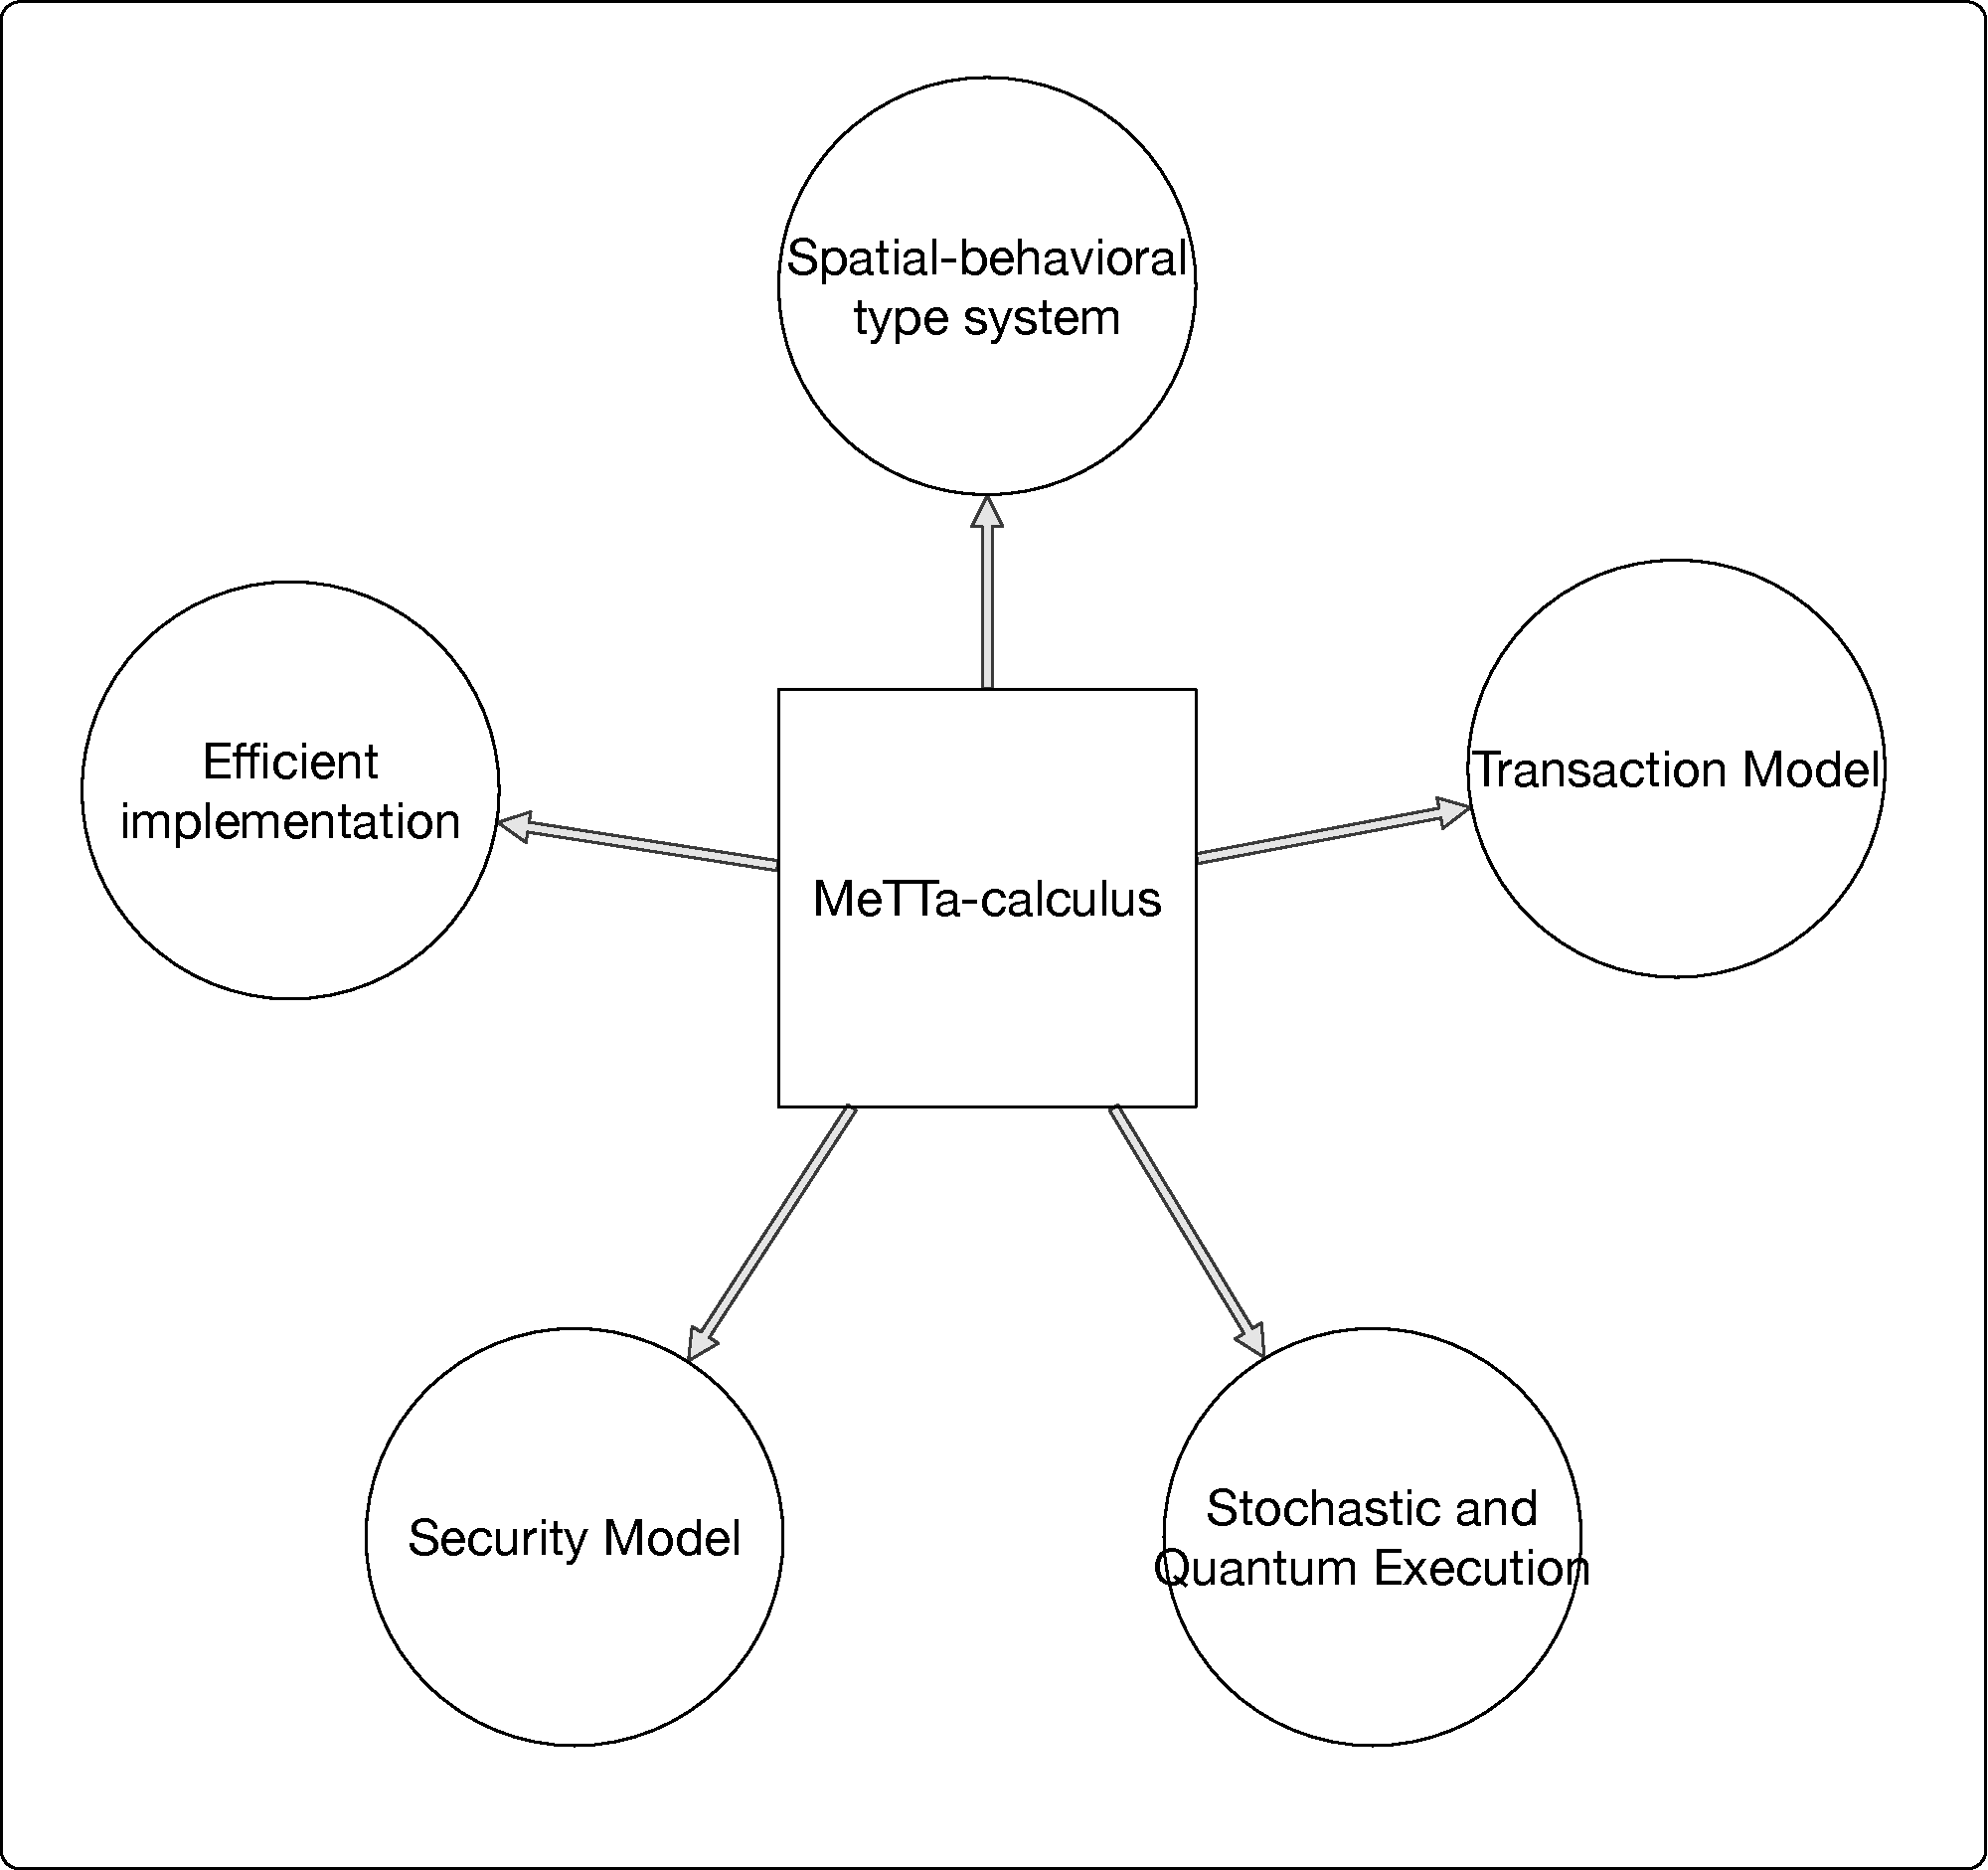
\includegraphics[scale=0.25]{MeTTaCalculusGenerationOfFeatures.pdf} \\
  \caption{Generating features from the $\mathsf{MeTTa}$-calculus}
\end{figure}

In general, presenting $\mathsf{MeTTa}$ as a graph structured lambda
theory, otherwise known as a structured operational semantics, not
only has the benefit that implementation follows the
correct-by-construction methodology, but may be used to automatically
derive and extend $\mathsf{MeTTa}$ with much needed features for
programming real applications in a distributed and decentralized
setting, as well as supporting well established programming paradigms,
such as semi-colon delimited sequential assignment programs.
 
 
%\section{Concurrent process calculi and spatial logics }\label{sec:concurrent_process_calculi_and_spatial_logics_} % (fold) 
In the last thirty years the \emph{process calculi} have matured into
a remarkably powerful analytic tool for reasoning about concurrent and
distributed systems, such as Internet communication, security, or
application protocols (\cite{DBLP:conf/popl/AbadiB02},
\cite{DBLP:conf/epew/BrownLM05}, \cite{DBLP:conf/fossacs/LaneveZ05}),
but also chemical reactions, and biological protocols such as cell
signaling regimes (\cite{DBLP:conf/psb/RegevSS01},
\cite{DBLP:journals/ipl/PriamiRSS01}.). Process-calculus-based
algebraic specification of computational processes began with Milner's
Calculus for Communicating Systems (CCS) \cite{DBLP:books/sp/Milner80}
and Hoare's Communicating Sequential Processes (CSP)
\cite{DBLP:books/ph/Hoare85}. Being largely influenced by the hardware
models of the time, these formalisms were based on a fixed
communication topology, where computational processes are considered
to be something like components soldered to a motherboard.

But as radio and cellular technologies, and protocols like
$\mathsf{TCP/IP}$ became popularized, this influenced the evolution of
these formalisms. In particular, the trend toward physical mobility of
computational devices gave rise to the mobile process calculi, called
so because they envisioned a network of computational processes
connected by a dynamic communication topology that evolves as the
processes compute. In a sense the computational processes contemplated
by these formalisms are mobile in much the same way as participants at
a conference who randomly bump into one another and trade mobile
numbers and email addresses, or molecules that randomly bump into one
another and exchange electrons. It was this innovation of mobility
that greatly expanded the scope of applicability of these formalisms.

Perhaps the most paradigmatic version of these calculi is Milner,
Parrow, and Walker's $\pi$-calculus
\cite{DBLP:journals/iandc/MilnerPW92a},
\cite{DBLP:journals/iandc/MilnerPW92b}, which Milner refined with
\cite{DBLP:journals/mscs/Milner92} and \cite{milner91polyadicpi}. In
the $\pi$-calculus the dominant metaphor is very much processes as
mobile agents (e.g., conference participants, or molecules) bumping
into one another exchanging channels over which they can
communicate. Yet, another equally compelling metaphor is that
processes are mobile agents swimming in various nested compartments or
membranes. These membranes are called \emph{ambients} because they
both surround and are surrounded by other ambients, but also because
they \emph{move}. That is, they can enter or exit one another are. In
this sense the membranes themselves are the computational
agents. These intuitions are formalized in Cardelli and Gordon's
ambient calculus \cite{DBLP:journals/tcs/CardelliG00}, and
considerably refined by Cardelli's brane calculi
\cite{DBLP:conf/cmsb/Cardelli04}.

Note that it is common practice in the mobile process calculi
literature to refer to channels as \emph{names} and in this note we
will use these terms interchangeably. In the more abstract setting of
that includes calculi like the ambient calculus where names are really
tags associated with mobile membranes this more generic moniker makes
sense. In both the $\pi$ and ambient calculi names are the means of
synchronization and rendezvous for mobile processes.

It is notable that to this day there is no fully abstract encoding of
the ambient calculus into the $\pi$-calculus, suggesting that the
ambient calculus is somehow more expressive than the
$\pi$-calculus. That said, expressivity is not always a benefit. It is
quite difficult to map the ambient style of computation to trustless
distributed Internet-based protocols. The expressivity requires a
great deal more coordination which, in turn, requires a great deal
more trust. Meanwhile, the $\pi$-calculus has a ready mapping onto a
wide range of Internet protocols, which i exploited vigorously in
building Microsoft's BizTalk Process Orchestration. And the rho
calculus has an even better mapping to Internet protocols, which i
exploited even more vigorously in building RChain and F1R3FLY.io.

\subsection{Hennessy-Milner and spatial logics, and session types}

Companion to these calculi are logics and type systems which enable
practitioners not only to reason about the correctness of individual
agents, or specific ensembles of agents, but also about entire classes
of agents, identified as the witnesses of logical formulae. These
began with the Hennessy-Milner logics which build on Kripke's
interpretation of modal logic \cite{milner91polyadicpi}. More
recently, these logics have been given new superpowers in the form of
being able to detect structural properties. Notably, we find Cardelli
and Caires's groundbreaking spatial logic
\cite{DBLP:conf/fossacs/Caires04} \cite{DBLP:journals/iandc/CairesC03}
\cite{DBLP:journals/tcs/CairesC04}. The interested reader might also
look at \emph{session types}
\cite{DBLP:conf/wsfm/Dezani-Ciancaglinid09}.

This topic is worthy of a much richer and deeper discussion. However,
we relegate that to a separate paper in which we unify them all with a
single algorithm, the $\mathsf{OSLF}$ algorithm. This takes as input a
model of computation formatted as a graph structured lambda theory and
outputs a spatial-behavioral type system for that model of
computation. The type system enjoys the Hennessy-Milner property,
namely that two computations inhabit the same bisimulation equivalence
class iff they satisfy exactly the same set of types. We leave the
details to the paper describing this algorithm.

\subsection{Compositionality and bisimulation}
Among the many reasons for the continued success of the mobile process
calculi's approach to organizing and analyzing computation are two
central points. First, the process algebras provide a compositional
approach to the specification, analysis and execution of concurrent
and distributed systems. Owing to Milner's original insights into
computation as interaction \cite{DBLP:journals/cacm/Milner93}, the
process calculi are so organized that the behavior ---the semantics---
of a system may be composed from the behavior of its components. This
means that specifications can be constructed in terms of components
---without a global view of the system--- and assembled into
increasingly complete descriptions.

The second central point is that process algebras have a potent proof
principle, yielding a wide range of effective and novel proof
techniques \cite{DBLP:conf/concur/SangiorgiM92}
\cite{DBLP:conf/fmco/Sangiorgi05}
\cite{DBLP:journals/toplas/Sangiorgi09}. In particular,
\emph{bisimulation} encapsulates an effective notion of process
equivalence that has been used in applications as far-ranging as
algorithmic games semantics \cite{DBLP:conf/sas/Abramsky05} and the
construction of model-checkers \cite{caires_2004}. The essential
notion can be stated in an intuitively recursive formulation: a
\emph{bisimulation} between two processes $P$ and $Q$ is an
equivalence relation $E$ relating $P$ and $Q$ such that: whatever
action of $P$ can be observed, taking it to a new state $P'$, can be
observed of $Q$, taking it to a new state $Q'$, such that $P'$ is
related to $Q'$ by $E$ and vice versa. $P$ and $Q$ are
\emph{bisimilar} if there is some bisimulation relating them. Part of
what makes this notion so robust and widely applicable is that it is
parameterized in the actions observable of processes $P$ and $Q$, thus
providing a framework for a broad range of equivalences and up-to
techniques \cite{DBLP:conf/concur/SangiorgiM92} all governed by the
same core principle \cite{DBLP:journals/toplas/Sangiorgi09}.

\section{The reflective higher order calculus}

It is in the context of the evolution of the mobile process calculi
that Meredith and Radestock's \emph{r}eflective
\emph{h}igher-\emph{o}rder, or rho calculus arises \footnote{The
$\pi$-calculus gets its name because it was the first Greek letter
available after the $\lambda$ in Church's calculus by that name, and
just happens to be the Greek letter corresponding to the English 'p'
for process. Likewise, the rho calculus gets its name from its
delivery of higher-order features through the use of reflection, and
it just happens that the acronym spells out \emph{rho}, the English
spelling of the Greek letter that comes after $\pi$.}
\cite{DBLP:journals/entcs/MeredithR05}. While it is possible to give a
faithful encoding of the ambient calculus into the rho calculus, the
rho calculus can be viewed as the natural successor to the
$\pi$-calculus. One way to look at the relationship between the two is
that the $\pi$-calculus is not actually a single calculus. Instead, it
is a recipe or \emph{function} for constructing a calculus of agents
that communicate over \emph{some} collection of channels. That is, it
is parametric in a \emph{theory} of channels\footnote{Note that here
we are using the term 'theory' in a technical sense, such as Peano
arithmetic, or a Lawvere theory. We don't mean theoretical in the
usual sense of that word, but rather a collection of entities (such as
the Natural Numbers) that can be generated from a small set of
rules.}. This intuition can be made very precise and corresponds to a
particular strategy of implementation called two-level type
decomposition. But, if the $\pi$-calculus is a function taking a
theory of channels to a theory of agents communicating over those
channels, then the rho calculus is the \emph{least fixed point} of
that function. The rho calculus says we need look no farther than the
\emph{communicating agent themselves} for our theory of channels.

More specifically, the calculus envisions a new kind of distinction,
one between the \emph{code} of a process, and a \emph{running
instance} of a process. It will not have escaped the reader's
attention that this is a commonplace notion in the practice of
building concurrent and distributed systems. Indeed, the development
of the rho calculus stole a page from the previous evolution of
process algebras. The step introducing mobility was the theory coming
into better alignment with practice. Computing devices became mobile,
to keep up the formalisms had to follow suit and devise a notion of
mobile processes. Likewise, the practice of building the software that
comprises concurrent and distributed systems makes a distinction
between code and running instances of the code. We argue, however,
that providing an account of this distinction in our formalism is much
more fundamental than just keeping up with practice. We argue that
this reason this is such a ubiquitous practice is because it is a
fundamental aspect of the underlying order and organization of
computation.

\subsection{Coding as a fundamental aspect of computation}

Indeed, G\"odel's incompleteness results fundamentally depend on
coding. To achieve the self-reference needed to construct a logical
statement of the form ``This sentence is not provable.'' G\"odel
encoded logical formulae into the natural numbers and then used
logical statements about the natural numbers to construct
self-referential statements like that one. In his construction, the
coding trick appears to be exogenous to logic and arithmetic, indeed a
careful study of these formalisms shows that it is, in fact,
\emph{intrinsic}. Moreover, this intrinsic, loopy self-reference that
arises from the notion of code is also at the heart of Turing's
solution to the Entscheidungsproblem and Cantor's separation of the
countably infinite from the uncountably infinite.

Moreover, the scope of this phenomenon is not restricted to some of
the most profound results in mathematics and logic over the last
couple of centuries. It's also at the heart of the origin of
life. Some four billion years ago chemistry stumbled on a way to code
for the production of proteins involved in certain self-replicating
chemical reactions. Arguments about the validity of the Weissman
barrier to one side \cite{William2018TheGA}, it is a matter of
experimentally established fact that the codons at the heart of the
genetic apparatus provide the mechanism for both the self-replication
of the chemical processes underlying life, but also the transmission
of inherited information about fitness to environment. As such, we
believe that coding is a much more profound phenomenon than has been
appreciated and deserves to be given a first-class representation in
our computational formalisms.

Once reflection is introduced into the mobile process calculus
setting, higher-order capabilities and recursion are child's
play. More surprisingly, so is the mysterious $\mathsf{new}$ operator
for generating fresh channels. But, we are getting ahead of
ourselves. Suffice it to say that using reflection as a first-class
representation of the trick of coding -- a trick originally discovered
by life and then independently rediscovered by Cantor, G\"odel, and
Turing -- is a real banger.

Intriguingly, not only does introducing coding explicitly into the
formalism solve a number of practical problems associated with the
$\pi$-calculus, it simultaneously solves a number of problems
associated with correspinding logics and type systems, as well. The
interested reader should see namespace logic
\cite{DBLP:conf/tgc/MeredithR05}.

\section{An idiosyncratic view of related work}

Here we direct the reader to a small sample of the considerable work
on the mobile process calculi. This sample is far from representative
of the overall body of work, but instead constitutes a snapshot of
what your author felt was salient at some point during the last twenty
years. Indeed, the reader is encouraged to investigate the literature
on her own to get an independent perspective on this rich field of
research.

\begin{itemize}
\item telecommunications, networking, security and application level protocols
\cite{DBLP:conf/popl/AbadiB02} 
\cite{DBLP:journals/tcs/AbadiB03} 
\cite{DBLP:conf/epew/BrownLM05} 
\cite{DBLP:conf/fossacs/LaneveZ05}; 
\item programming language semantics and design
\cite{DBLP:conf/epew/BrownLM05}
\cite{djoin}
\cite{DBLP:conf/afp/FournetFMS02}
\cite{DBLP:journals/toplas/SewellWU10};
\item webservices
\cite{DBLP:conf/epew/BrownLM05}
\cite{DBLP:conf/fossacs/LaneveZ05}
\cite{DBLP:conf/wise/Meredith03};
\item{blockchain}
  \cite{meredith_2017}
\item and biological systems
\cite{DBLP:conf/cmsb/Cardelli04}
\cite{DBLP:conf/esop/DanosL03}
\cite{DBLP:conf/psb/RegevSS01}
\cite{DBLP:journals/ipl/PriamiRSS01}.
\end{itemize}


% section concurrent_process_calculi_and_spatial_logics_ (end)


%\section{The syntax and semantics of the core rho calculus}\label{sub:the_syntax_and_semantics_of_the_notation_system} % (fold)

We now summarize a technical presentation of the core calculus. The
typical presentation of such a calculus generalizes a generators and
relations presentation of an algebra
\cite{nlab:generators_and_relations}. The grammar below, describing
term constructors in the language of process expressions (which we
abbreviate to processes in the sequel), freely generates the set of
processes. We denote this set $\Proc$, and the set of channels (aka
names) over which these processes communicate by $\QProc$. The set
$\Proc$ (and by extension $\QProc$) is then quotiented by a relation
known as structural congruence, denoted $\equiv$, and it is over this
set that the notion of computation is expressed.

In particular, computation is expressed as a small handful of rewrite
rules which should be viewed as defining a state transition
relation. Thus, process expressions capture \emph{states} and the form
of the expression determines how one process (state) \emph{might}
evolve to another (state). The word 'might' is doing some heavy
lifting in that previous sentence, as the calculus is \emph{not}
deterministic, in fact it is not even confluent. As such, the calculus
can be used to represent all manner of common human (and natural)
resource distribution protocols, such as first come first served,
which sits at the heart of everything from airline reservation systems
to concert ticket sales. By comparison, Church's $\lambda$-calulus
(the core of programming languages such as $\mathsf{Haskell}$ or
$\mathsf{Scala}$) does not -- without considerable modification --
natively support the expression of such protocols.

\subsection{The rho calculus in less than a page}

\begin{mathpar}
\inferrule* [lab=process] {} {P, Q \bc \pzero \;\bm\; \mathsf{for}(
  y \leftarrow x )P \;\bm\; x\mathsf{!}(Q) \;\bm\;
  \mathsf{*}x \;\bm\; P\mathsf{|}Q } \and \inferrule* [lab=name] {}
            {x, y \bc \mathsf{@}P }
\end{mathpar}

\begin{mathpar}
  \inferrule* [lab=equiv] {} {P\mathsf{|}\pzero \equiv P \;\; P\mathsf{|}Q \equiv Q\mathsf{|}P \;\; P\mathsf{|}(Q\mathsf{|}R) \equiv (P\mathsf{|}Q)\mathsf{R}} \\
  \and
  \inferrule* [lab=alpha] {} {\mathsf{for}(y \leftarrow x )P \equiv \mathsf{for}(z \leftarrow x )(P\{z/y\} \; \mathsf{if} z \notin \mathsf{FN}(P)}
\end{mathpar}

\begin{mathpar}
  \inferrule* [lab=COMM] {} {\mathsf{for}( y \leftarrow x )P \;\mathsf{|}\; x!(\arrvec{Q})
    \red P\substn{\quotep{Q}}{y}} \\
  %% \and
  %% \inferrule* [lab=PAR]{P \red P'}{P\mathsf{|}Q \red P'\mathsf{|}Q}
  %% \and
  %% \inferrule* [lab=EQUIV]{{P \;\scong\; P'} \andalso {P' \red Q'} \andalso {Q' \;\scong\; Q}}{P \red Q}
\end{mathpar}

This presentation is essentially that of
\cite{DBLP:journals/entcs/MeredithR05} recast with a
programmer-friendly syntax that extends smoothly to fork-join patterns
commonly found in human decision-making processes. The reader should
note that, even with a programmer-friendly syntax, this calculus is
considerably smaller than a corresponding presentation of the
$\pi$-calculus. Indeed is as concise and compact as the
$\lambda$-calculus, yet considerably more expressive. What follows
below is an exegesis of the technical details hidden in this more
compact presentation. Notably, we provide definitions of free and
bound names, we add two more rewrite rules that prescribe how rewrites
may occur in context (necessary, since the calculus is not
deterministic) and other housekeeping matters such as name
equality. The reader more familiar with these notions should feel free
to skim this section, however the section on bisimulation is of some
importance and worthy of more focused attention.

\subsection{The fine print}

\paragraph{Notational interlude} when it is clear that some expression $t$ is a sequence (such as a list or a vector), and $a$ is an object that might be meaningfully and safely prefixed to that sequence then we write $a:t$ for the sequence with $a$ prefixed (aka ``consed'') to $t$. We write $t(i)$ for the $i$th element of $t$. In the sequel we use $\arrvec{x}$ (resp. $\arrvec{P}$) denotes a vector of \emph{names}
(resp. \emph{processes}) of length $|\arrvec{x}|$
(resp. $|\arrvec{P}|$).

\subsubsection{Process grammar}\label{subsub:process_grammar}

\begin{mathpar}
\inferrule* [lab=process] {} {P, Q \bc \pzero \;\bm\; \mathsf{for}(
  y \leftarrow x )P \;\bm\; x\mathsf{!}(Q) \;\bm\;
  \mathsf{*}x \;\bm\; P\mathsf{|}Q } \and \inferrule* [lab=name] {}
            {x, y \bc \mathsf{@}P }
\end{mathpar}

As mentioned above we use $\Proc$ (resp. $\QProc$) to denote the
language of processes (resp. names) freely generated by this
grammar. But how are we to think about expressions in this language,
intuitively?

\begin{itemize}
  \item $\pzero$ is the ground of this tiny little language. It represents the \emph{stopped} process, or the process that does nothing; in some real sense this is the quintessential neutral element in this computational dynamics, as we shall see;
  \item $\mathsf{for}( y \leftarrow x )P$ is the process that is waiting at channel $x$ for some data or message that it will bind to $y$ and then proceed to do $P$; if $\pzero$ is neutral, then $\mathsf{for}$-comprehension is receptive, it waits for action at $x$ before it can do anything;
  \item $x\mathsf{!}(Q)$ is the process that is outputting the datum or message $Q$ (which is also a process) along the channel, $x$; if $\pzero$ is neutral, and $\mathsf{for}( y \leftarrow x )P$ is reception, then $x\mathsf{!}(Q)$ is active; it represents actively sending $Q$ floating down the channel $x$ to be picked up by some $\mathsf{for}( y \leftarrow x )P$;
  \item $\mathsf{*}x$ is the process that takes the code represented by $x$ and begins running it;
  \item $P\mathsf{|}Q$ is the process that is the parallel or concurrent composition of the process $P$ with the process $Q$; it introduces the principle that individual computations can actually be collectives of autonomous, yet coordinating computation.  
\end{itemize}

As foreshadowed by the syntactic category of expressions of the form
$\mathsf{*}x$, a channel or name is merely the code of some process,
$\mathsf{@}P$. In this sense we may think of these two operators
$\mathsf{*}$ and $\mathsf{@}$ as dual to one another. The latter
delivers the code of some process, while the former delivers a running
process from its code.

Next, we quotient this set by the smallest equivalence
relation containing $\alpha$-equivalence that makes $(\Proc, |, 0)$
into a commutative monoid. In order to define this relation we require
a definition of free and bound names to define $\alpha$-equivalence.

\begin{definition}
  \emph{Free and bound names} The calculation of the free names of a
  process, $P$, denoted $\freenames{P}$ is given recursively by
  
  \begin{mathpar}
    \freenames{\pzero} = \emptyset
    \and
    \freenames{\mathsf{for}(y \leftarrow x)(P)} = \{ x \} \cup \freenames{P}\setminus\{y\}
    \and
    \freenames{x!(P)} = \{ x \} \cup \freenames{P}
    \and
    \freenames{P|Q} = \freenames{P} \cup \freenames{Q}
    \and
    \freenames{\mathsf{}{x}} = \{ x \} \\
  \end{mathpar}
  
  An occurrence of $x$ in a process $P$ is \textit{bound} if it is not
  free. The set of names occurring in a process (bound or free) is
  denoted by $\names{P}$.
\end{definition}

\subsection{Substitution}

We use the notation $\id{\{}\arrvec{y} / \arrvec{x} \id{\}}$ to denote
partial maps, $s : \QProc \rightarrow \QProc$. A map, $s$ lifts,
uniquely, to a map on process terms, $\widehat{s} : \Proc \rightarrow
\Proc$. Historically, it is convention to use $\sigma$ to range over
lifted subsitutions, $\widehat{s}$, to write the application of a
substitution, $\sigma$ to a process, $P$, using postfix notation, with
the substitution on the right, $P\sigma$, and the application of a
substitution, $s$, to a name, $x$, using standard function application
notation, $s(x)$. In this instance we choose not to swim against the
tides of history. Thus,

\begin{definition}
  given $x = \quotep{P'}$, $u = \quotep{Q'}$, $s =
  \substn{u}{x}$ we define the lifting of $s$ to $\widehat{s}$ (written
  below as $\sigma$) recursively by the following equations.
  \begin{mathpar}
    0 \sigma := 0 \\
    (P \mathsf{|} Q) \sigma
    :=    
    P\sigma \mathsf{|} Q\sigma \\
    (\mathsf{for}(y \leftarrow v)P) \sigma    
    :=
    \mathsf{for}(z \leftarrow \sigma(v))((P \psubstn{z}{y}) \sigma) \\
    (\lift{x}{Q}) \sigma  
    :=
    \lift{\sigma(x)}{ Q \sigma } \\
    (\dropn{y})  \sigma       
    := 
    \left\{ 
      \begin{array}{ccc} 
        Q' & & y \;\nameeq\; x \\
        \dropn{y} & & otherwise \\
      \end{array}
      \right.
  \end{mathpar} 

  where

  \begin{eqnarray}
    \psubstp{Q}{P}(x) = \id{\{} \quotep{Q} / \quotep{P} \id{\}}(x) = 
    \left\{ 
      \begin{array}{ccc}
        \quotep{Q} & & x \;\nameeq\; \quotep{P} \\
        x & & otherwise \\
      \end{array}
      \right. \nonumber
  \end{eqnarray}
\end{definition}

and $z$ is chosen distinct from $\quotep{P}$, $\quotep{Q}$, the free
names in $Q$, and all the names in $R$. Our $\alpha$-equivalence will
be built in the standard way from this substitution.

\begin{definition}
Then two processes, $P,Q$, are alpha-equivalent if $P = Q\{\arrvec{y}/\arrvec{x}\}$ for
some $\arrvec{x} \in \boundnames{Q},\arrvec{y} \in \boundnames{P}$, where $Q\{\arrvec{y}/\arrvec{x}\}$
denotes the capture-avoiding substitution of $\arrvec{y}$ for $\arrvec{x}$ in $Q$.
\end{definition}

\begin{definition}
  The {\em structural congruence} $\equiv$
  between processes \cite{DBLP:books/daglib/0004377} is the least congruence containing
  alpha-equivalence and satisfying the commutative monoid laws
  (associativity, commutativity and $\pzero$ as identity) for parallel
  composition $|$.
\end{definition}

\begin{definition}
  The {\em name equivalence} $\nameeq$ is the least congruence
  satisfying these equations
  \begin{mathpar}
  \inferrule*[lab=Quote-drop] {}{ \quotep{\dropn{x}} \;\nameeq\; x }
  \and
  \inferrule*[lab=Struct-equiv] { P \;\scong\; Q } { \quotep{P} \;\nameeq\; \quotep{Q} }
  \end{mathpar}
\end{definition}

The astute reader will have noticed that the mutual recursion of names
and processes imposes a mutual recursion on alpha-equivalence and
structural equivalence via name-equivalence. Fortunately, all of this
works out pleasantly and we may calculate in the natural way, free of
concern. The reader interested in the details is referred to the
appendix \ref{appendix:rho_details}.

\begin{remark}\label{rem:no_self_referential_names}
  One particularly useful consequence of these definitions is that
  $\forall P. \quotep{P} \not\in \freenames{P}$. It gives us a
  succinct way to construct a name that is distinct from all the names
  in $P$ and hence fresh in the context of $P$. For those readers
  familiar with the work of Pitts and Gabbay, this consequence allows
  the system to completely obviate the need for a fresh operator, and
  likewise provides a canonical approach to the semantics of
  freshness.
\end{remark}

Equipped with the structural features of the term language we can
present the dynamics of the calculus.

\subsection{Operational semantics}

Finally, we introduce the computational dynamics. What marks these
algebras as distinct from other more traditionally studied algebraic
structures, e.g. vector spaces or polynomial rings, is the manner in
which dynamics is captured. In traditional structures, dynamics is typically
expressed through morphisms between such structures, as in linear maps
between vector spaces or morphisms between rings. In algebras
associated with the semantics of computation, the dynamics is
expressed as part of the algebraic structure itself, through a
reduction reduction relation typically denoted by $\red$. Below, we
give a recursive presentation of this relation for the calculus used
in the encoding.

\begin{mathpar}
  \inferrule* [lab=COMM] {x_{t} \;\nameeq\; x_{s}} {\mathsf{for}( y \leftarrow x_{t} )P \;\mathsf{|}\; x_{s}!(\arrvec{Q})
  \red P\substn{\quotep{Q}}{y}}
  \and
  \inferrule* [lab=PAR]{P \red P'}{P\mathsf{|}Q \red P'\mathsf{|}Q}
  \and
  \inferrule* [lab=EQUIV]{{P \;\scong\; P'} \andalso {P' \red Q'} \andalso {Q' \;\scong\; Q}}{P \red Q}
\end{mathpar}

We write $P\red$ if $\exists Q $ such that $ P \red Q$ and $P\not\red$, otherwise.

\subsection{ Dynamic quote: an example }

Anticipating something of what's to come, let $z = \quotep{P}$, $u = \quotep{Q}$, and $x = \quotep{\lift{y}{\dropn{z}}}$. Now consider applying the substitution,
$\widehat{\id{\{}u / z \id{\}}}$, to the following pair of processes,
$\lift{w}{y!(\dropn{z})}$ and $\lift{w}{\dropn{x}} = \lift{w}{\dropn{\quotep{\lift{y}{\dropn{z}}}}}$.

\begin{eqnarray}
	\lift{w}{\lift{y}{\dropn{z}}}\widehat{\id{\{}u / z \id{\}}}
		& = &
		\lift{w}{\lift{y}{Q}} \nonumber\\
	\lift{w}{\dropn{x}} \widehat{ \id{\{}u / z \id{\}} }
		& = &
		\lift{w}{\dropn{x}} \nonumber
\end{eqnarray}

The body of the quoted process, $\quotep{\lift{y}{\dropn{z}}}$, is
impervious to substitution, thus we get radically different
answers. In fact, by examining the first process in an input context,
e.g. $\mathsf{for}(z \leftarrow x)\lift{w}{\lift{y}{\dropn{z}}}$, we see that the process
under the output operator may be shaped by prefixed inputs binding a
name inside it. In this sense, the combination of input prefix binding
and output operators will be seen as a way to dynamically construct
processes before reifying them as names.

\section{Replication}

As mentioned before, it is known that replication (and hence
recursion) can be implemented in a higher-order process algebra
\cite{DBLP:books/daglib/0004377}. As our first example of calculation with the
machinery thus far presented we give the construction explicitly in
the rho calculus.

\begin{eqnarray}
	D_{x} & := & \prefix{x}{y}{(\binpar{\outputp{x}{y}}{\dropn{y}})} \nonumber\\
	\bangp_{x}{P} & := & \binpar{\lift{x}{\binpar{D_{x}}{P}}}{D_{x}} \nonumber
\end{eqnarray}

\begin{eqnarray}
	\bangp_{x}{P} & & \nonumber\\
	=
	& \lift{x}{(\prefix{x}{y}{(\outputp{x}{y} | \dropn{y})) | P}} 
	      | \prefix{x}{y}{(\outputp{x}{y} | \dropn{y})} & \nonumber\\
	\red
	& (\outputp{x}{y} | \dropn{y})\substn{\quotep{(\prefix{x}{y}{(\dropn{y} | \outputp{x}{y})) | P}}}{y} & \nonumber\\
	=
	& \outputp{x}{\quotep{(\prefix{x}{y}{(\outputp{x}{y} | \dropn{y})) | P}}}
	  | {(\prefix{x}{y}{(\outputp{x}{y} | \dropn{y})) | P}} & \nonumber\\
	\red
	& \ldots & \nonumber\\
	\red^*
	& P | P | \ldots & \nonumber
\end{eqnarray}

Of course, this encoding, as an implementation, runs away, unfolding
$\bangp{P}$ eagerly. A lazier and more implementable replication
operator, restricted to input-guarded processes, may be obtained as follows.

\begin{eqnarray}
\bangp{\prefix{u}{v}{P}} 
	:= 
	\binpar{\lift{x}{\prefix{u}{v}{(\binpar{D(x)}{P})}}}{D(x)} \nonumber
\end{eqnarray}

\begin{remark}
  Note that the lazier definition still does not deal with summation
  or mixed summation (i.e. sums over input and output). The reader is
  invited to construct definitions of replication that deal with these
  features. 

  Further, the definitions are parameterized in a name, $x$. Can you,
  gentle reader, make a definition that eliminates this parameter and
  guarantees no accidental interaction between the replication
  machinery and the process being replicated -- i.e. no accidental
  sharing of names used by the process to get its work done and the
  name(s) used by the replication to effect copying. This latter
  revision of the definition of replication is crucial to obtaining
  the expected identity $!!P \sim !P$.
\end{remark}

\begin{remark}\label{rem:paradoxical_combinator}
  The reader familiar with the lambda calculus will have noticed the
  similarity between $D$ and the paradoxical combinator.

  [Ed. note: the existence of this seems to suggest we have to be more
  restrictive on the set of processes and names we admit if we are to
  support no-cloning.]
\end{remark}

\subsubsection{Bisimulation}

The computational dynamics gives rise to another kind of equivalence,
the equivalence of computational behavior. As previously mentioned
this is typically captured \emph{via} some form of bisimulation.

% The notion we use in this paper is weak barbed bisimulation
% \cite{milner91polyadicpi}.

The notion we use in this paper is derived from weak barbed
bisimulation \cite{milner91polyadicpi}. 

\begin{definition}
An \emph{observation relation}, $\downarrow_{\mathcal N}$, over a set
of names, $\mathcal N$, is the smallest relation satisfying the rules
below.

\infrule[Out-barb]{y \in {\mathcal N}, \; x \nameeq y}
		  {\outputp{x}{v} \downarrow_{\mathcal N} x}
\infrule[Par-barb]{\mbox{$P\downarrow_{\mathcal N} x$ or $Q\downarrow_{\mathcal N} x$}}
		  {\binpar{P}{Q} \downarrow_{\mathcal N} x}

We write $P \Downarrow_{\mathcal N} x$ if there is $Q$ such that 
$P \wred Q$ and $Q \downarrow_{\mathcal N} x$.
\end{definition}

\begin{definition}
%\label{def.bbisim}
An  ${\mathcal N}$-\emph{barbed bisimulation} over a set of names, ${\mathcal N}$, is a symmetric binary relation 
${\mathcal S}_{\mathcal N}$ between agents such that $P\rel{S}_{\mathcal N}Q$ implies:
\begin{enumerate}
\item If $P \red P'$ then $Q \wred Q'$ and $P'\rel{S}_{\mathcal N} Q'$.
\item If $P\downarrow_{\mathcal N} x$, then $Q\Downarrow_{\mathcal N} x$.
\end{enumerate}
$P$ is ${\mathcal N}$-barbed bisimilar to $Q$, written
$P \wbbisim_{\mathcal N} Q$, if $P \rel{S}_{\mathcal N} Q$ for some ${\mathcal N}$-barbed bisimulation ${\mathcal S}_{\mathcal N}$.
\end{definition}

\subsubsection{Contexts}

One of the principle advantages of computational calculi from the
$\lambda$-calculus to the $\pi$-calculus is a well-defined notion of context,
contextual-equivalence and a correlation between
contextual-equivalence and notions of bisimulation. The notion of
context allows the decomposition of a process into (sub-)process and
its syntactic environment, its context. Thus, a context may be
thought of as a process with a ``hole'' (written $\Box$) in it. The
application of a context $K$ to a process $P$, written $K[P]$, is
tantamount to filling the hole in $K$ with $P$. In this paper we do
not need the full weight of this theory, but do make use of the notion
of context in the proof the main theorem. 

\begin{mathpar}
\inferrule* [lab=context] {} {K \bc \Box \;\bm\; \mathsf{for}( \arrvec{y} \leftarrow x )K \;\bm\; x\mathsf{!}(\arrvec{P},K,\arrvec{Q}) \;\bm\; K\mathsf{|}P }
\end{mathpar}

\begin{definition}[contextual application] Given a context $K$, and
  process $P$, we define the \emph{contextual application}, $K[P] :=
  K\{P/\Box\}$. That is, the contextual application of K to P is the
  substitution of $P$ for $\Box$ in $K$.
\end{definition}

\begin{remark}
  Note that we can extend the definition of free and bound names to contexts.
\end{remark}

% subsection the_syntax_and_semantics_of_the_notation_system (end)   


%\section{Implementing rho calculus on modern computers}

\subsection{RSpace: a new kind of key-value store}

TBD

\subsection{Compiling rho to RSpace}

\subsubsection{Ordering rho terms}

TBD


%\section{Useful syntactic sugar}

\subsection{First class values}
While it is standard in calculi such as the $\lambda$-calculus to
define a variety of common values such as the natural numbers and
booleans in terms of Church-numeral style encodings, it is equally
common to simply embed values directly into the calculus. Not being
higher-order, this presents some challenges for the $\pi$-calculus,
but for the rho-calculus, everything works out very nicely if we treat
values, e.g. the naturals, the booleans, the reals, etc as processes. This
choice means we can meaninfully write expressions like
$x!(\mathsf{5})$ or $u!(\mathsf{true})$, and in the context
$\prefix{x}{y}P[*y] \mathsf{|} x!(\mathsf{5})$ the value $\mathsf{5}$
will be substituted into $P$. Indeed, since operations like addition,
multiplication, etc.  can also be defined in terms of processes, it is
meaningful to write expressions like
$\mathsf{5}\mathsf{|}\mathsf{+}\mathsf{|}\mathsf{1}$, and be confident
that this expression will reduce to a process representing
$\mathsf{6}$. Thus, we can also use standard mathematical expressions,
such as $\mathsf{5+1}$, as processes, and know that these will
evaluate to their expected values. Further, when combined with
$\mathsf{for}$-comprehensions, we can write algebraic expressions,
such as $\prefix{x}{y}\mathsf{5}\mathsf{+}\mathsf{*}y$, and in
contexts like
$(\prefix{x}{y}\mathsf{5}\mathsf{+}\mathsf{*}y)\mathsf{|}\outputp{x}{\mathsf{1}}$
this will evaluate as expected, producing the process (aka value)
$\mathsf{6}$.

\begin{mathpar}
  \inferrule* [lab=values] {} {\mathsf{Proc} \bc \dots \bm \mathsf{Bool}
    \bm \mathsf{Long}
    \bm \mathsf{String}
    \bm \mathsf{Uri} \bm \mathsf{Collection} \bm \ldots}
\end{mathpar}

\begin{mathpar}
  \inferrule* [lab=collection] {} {\mathsf{Collection} \bc \texttt{[} \mathsf{[}\mathsf{Proc}\mathsf{]} \texttt{]}
    \bm \texttt{(} \mathsf{Proc} \texttt{,}\; \mathsf{[}\mathsf{Proc}\mathsf{]} \texttt{)}
    \bm \texttt{Set} \texttt{(} \mathsf{[}\mathsf{Proc}\mathsf{]} \texttt{)}
    \bm \texttt{\{} \mathsf{[}\mathsf{Proc} \texttt{:} \mathsf{Proc} \mathsf{]} \texttt{\}}} \\
\end{mathpar}

\subsection{Pattern matching}
Remember that rho allows processes to be sent: $x\mathsf{!}(Q)$. Since
we can send values, it will be useful to be able to pattern match on
values. The following pattern-matching syntax captures very commonly
used idioms.

\subsubsection{Patterns}
\begin{mathpar}
  \inferrule* [lab=pattern] {} {\mathsf{ProcPattern} \bc \texttt{\_}
    \bm \mathsf{Var}
    \bm \texttt{@} \mathsf{ProcPattern}
    \bm\; \mathsf{VarRefKind}\; \mathsf{Var} \bm \mathsf{LogicalPattern} \bm \mathsf{ValuePattern}} \\
  \and
  \inferrule* [lab=logical-pattern] {} {\mathsf{LogicalPattern} \bc \mathsf{ProcPattern} \;\vee\; \mathsf{ProcPattern}
    \bm \mathsf{ProcPattern} \;\wedge\; \mathsf{ProcPattern}
    \bm \texttt{\~{}} \mathsf{ProcPattern}} \\
  \and
  \inferrule* [lab=value-pattern] {} {\mathsf{ValuePattern} \bc \mathsf{Ground}
    \bm \mathsf{Collection}
    \bm \texttt{Nil}
    \bm \mathsf{SimpleType}} \\
  \and
  \inferrule* [lab=var-ref-kind] {} {\mathsf{VarRefKind} \bc \texttt{=} \bm \texttt{=} \texttt{*}} \\
\end{mathpar}

\subsubsection{Match targets}

Match targets are the syntactic contexts where patterns may occur and
thus generate substitutions to be applied in the sequel.

\begin{mathpar}
  \inferrule* [lab=match-targets] {} {\mathsf{Proc} \bc \ldots \;\bm\; \texttt{contract}\; \mathsf{Name}\; \texttt{(} \mathsf{[Name]}\; \mathsf{NameRemainder} \texttt{)}\; \texttt{=}\; \texttt{\{}\; \mathsf{Proc}\; \texttt{\}} \\
    \and
    \;\bm\; \texttt{for}\; \texttt{(} \mathsf{[Receipt]} \texttt{)} \texttt{\{} \;\mathsf{Proc}\; \texttt{\}} \;\bm\; \texttt{select}\; \texttt{\{} \;\mathsf{[Branch]}\; \texttt{\}} \\
    \and
    \;\bm\; \texttt{match}\; \mathsf{Proc}\; \texttt{\{} \;\mathsf{[Case]}\; \texttt{\}} \;\bm\; \texttt{let}\; \mathsf{Decl}\; \mathsf{Decls}\; \texttt{in}\; \texttt{\{} \;\mathsf{Proc}\; \texttt{\}} }\\
\end{mathpar}

\subsubsection{Contracts}

Contracts provide for recursive definitions of processes.

\subsubsection{Comprehensions}

Comprehensions become considerably enriched. They are not only the
place where data can be matched, but also the place where we introduce
more subtle control flow. As such, we deal with those together in the
section on joins.

\subsubsection{Select}

Select represents guarded summation.

\subsubsection{Match}

Match allows dispatch on value shape without incurring the cost of synchronization.

\subsubsection{Let}

Let allows binding without incurring the cost of synchronization.

%% \subsection{Let syntax}
%% We achieve even greater compression and a more
%% familiar notation if we also adopt the notation

%% \begin{mathpar}
%%   \mathsf{let}\; x \;\mathsf{=}\; v \;\mathsf{in}\; P := (\mathsf{new} \; u)(\prefix{u}{@x}P)\mathsf{|}\outputp{u}{v}
%% \end{mathpar}
\subsection{Joins}

The basic template for joins is:

\begin{lstlisting}[mathescape=true]
  for(
    y$_{11}$ $\sngllarrow$ x$_{11}$ & $\ldots$ & y$_{m1}$ $\sngllarrow$ x$_{m1}$ ; // received in any order, 
       $\dots$ ; // but all received before the next row
    y$_{1n}$ $\sngllarrow$ x$_{1n}$ & $\ldots$ & y$_{mn}$ $\sngllarrow$ x$_{mn}$
  ){ $\ldots$ }
\end{lstlisting}

We extend this template to include not only linear consumption of
output ($y \;\sngllarrow\; x$); but also reads ($y \;\dblhdlarrow\;
x$), where the data is not consumed, but merely copied; and
subscriptions ($y \;\dbltllarrow\; x$) where the continuation is not
consumed, but a copy forked off.

Additionally, we add syntax for synchronous interaction. We
distinguish $y \;\sngllarrow\; x\texttt{?!}$ which is paired with ();
and $y \;\sngllarrow\; x\texttt{!?}( \ldots )$ the equivalent of an
remote procedure call (rpc).

\begin{mathpar}
  \inferrule* [lab=joins] {} {\mathsf{Proc2} \bc \mathsf{Proc3} \;\bm\; \;\ldots\; \;\bm\; \texttt{for}\; \texttt{(} \mathsf{[Receipt]} \texttt{)} \texttt{\{} \;\mathsf{Proc}\; \texttt{\}}} \\
    \and
  \inferrule* [lab=] {} {\mathsf{Receipt} \bc \mathsf{[LinearBind]} \;\bm\; \mathsf{[RepeatedBind]} \;\bm\; \mathsf{[PeekBind]}} \\
  \inferrule* [lab=] {} {\mathsf{[Receipt]} \bc \mathsf{Receipt} \;\bm\; \mathsf{Receipt} \;\texttt{;}\; \mathsf{[Receipt]}} \\
  \inferrule* [lab=] {} {\mathsf{LinearBind} \bc \mathsf{[Name]} \; \mathsf{NameRemainder} \;\sngllarrow\; \mathsf{NameSource}} \\
  \inferrule* [lab=] {} {\mathsf{[LinearBind]} \bc \mathsf{LinearBind} \;\bm\; \mathsf{LinearBind} \;\texttt{\&}\; \mathsf{[LinearBind]}} \\
  \inferrule* [lab=] {} {\mathsf{NameSource} \bc \mathsf{Name} \;\bm\; \mathsf{Name} \texttt{?!}\;\bm\; \mathsf{Name} \texttt{!?} \texttt{(} \mathsf{[Proc]} \texttt{)}} \\
  \inferrule* [lab=] {} {\mathsf{RepeatedBind} \bc \mathsf{[Name]}\; \mathsf{NameRemainder} \;\dbltllarrow\; \mathsf{Name}} \\
  \inferrule* [lab=] {} {\mathsf{[RepeatedBind]} \bc \mathsf{RepeatedBind} \;\bm\; \mathsf{RepeatedBind} \texttt{\&} \mathsf{[RepeatedBind]}} \\
  \inferrule* [lab=] {} {\mathsf{PeekBind} \bc \mathsf{[Name]}\; \mathsf{NameRemainder} \;\dblhdlarrow\; \mathsf{Name}} \\
  \inferrule* [lab=] {} {\mathsf{[PeekBind]} \bc \mathsf{PeekBind} \;\bm\; \mathsf{PeekBind} \;\texttt{\&}\; \mathsf{[PeekBind]}} \\
\end{mathpar}

\subsection{Unguessable versus unforgeable names}
Since all the names of the rho calculus are generated from the codes
of processes we know all of them up front. Security on channels,
therefore, amounts to unguessability. There are an infinite number of
names and we have to arrange our protocols to make it very, very hard
to guess which channels are in use at any given time. On the one hand,
we could delegate that to some black box which delivers us the next
unguessable name when we ask for it. In this sense, it is therefore
useful to reintroduce the $\pi$-calculus' $\mathsf{new}$ operator as a
standin for that black box.

However, in many settings, such as in the $\mathsf{RChain}$ and
$\mathsf{F1R3FLY.io}$ implementations execution is arranged so that
names are not merely unguessable, but \emph{unforgeable}, meaning that
the execution environment guarantees not to allow outside agents to
generate certain names. Thus, even if some malefactor guesses a
particular name, it cannot eavesdrop on the channel associated with it
because it can't execute code that uses that name because it didn't
have the right to generate it. It could only do so had its code been
in a scope where the generated name was sent to it by a (presumably)
willing party.

Thus, the $\mathsf{new}$ operator not only provides useful abstraction
over a black boxed unguessability algorithm, but can also be used to
support unforgeability. Hence, we reintroduce to rho as a conservative
extension.

\begin{mathpar}
  \inferrule* [lab=unforgeable] {} {P \bc \ldots \bm \texttt{new}\; \mathsf{[NameDecl]}\; \texttt{in}\; P} \\
  \and
  \inferrule* [lab=] {} {\mathsf{NameDecl} \bc \mathsf{Var} \bm \mathsf{Var} \texttt{(} \mathsf{Uri} \texttt{)}} \\
  \and
  \inferrule* [lab=] {} {\mathsf{[NameDecl]} \bc \mathsf{NameDecl} \bm \mathsf{NameDecl} \texttt{,} \mathsf{[NameDecl]}} \\
\end{mathpar}

\subsection{Summation}

\subsubsection{Mixed summation}
The presentation given so far is often referred to as the monadic,
asynchronous version of the rho-calculus. There is a natural polyadic
version, in which send and receive result in an exchange of a tuple of
processes. Further there is a natural extension in which we recognize
that certain processes can be made to behave like values and can
therefore be replaced by more familiar representations of those
values, and on top of this extension it becomes natural and compelling
to add pattern-matching to send and receive.

All of these extensions, which we will explore in some detail in the
subsequent sections, really only constitute syntactic sugar. Values,
pattern-matching, let expressions, and more can be desugared back down
to the original calculus. However, summation, aka non-deterministic
choice, where a process is in a superposition of states that get
``collapsed'' through interaction with and environment, affords
versions of the calculus that significantly extend the expressive
power of the calculus.

Specifically, mixed summation, or non-deterministic choice over both
guarded input ($\mathsf{for}$-comprehension) and output is not merely
a conservative extension of the calculus. Although there is an
encoding of the calculus with mixed summation to the asynchronous
calculus, it is not par-preserving. That is, if $\meaningof{-}_{async}
: \MixSumProc \to \Proc$ is a mapping from the rho-calculus with mixed
summation to the asynchronous polyadic rho-calulus, then it cannot be
the case that

\begin{mathpar}
  \meaningof{P\mathsf{|}Q}_{async} = \meaningof{P}_{async}\mathsf{|}\meaningof{Q}_{async}
\end{mathpar}

for any such encoding. For good measure we throw in synchronous
communication, but it is the mixed summation that constitutes the real
jump in expressive power. These features are useful when dealing with
probabilistic exection for both stochastic and quantum regimes. When
relating our model of concurrent computation to these other notions it
is important to track the points where there are significant increases
in expressive power of our target language.

Because Milner's presentation of the polyadic $\pi$-calculus
with mixed summation is so parsimonious we use it as a template for a
similar version of the rho-calculus.

\begin{mathpar}
  \inferrule* [lab=summation] {} {{M,N} \bc \pzero \;|\; x.A \;|\; M+N}
  \and
  \inferrule* [lab=agent] {} {A \bc (\arrvec{x})P \;| \; [\arrvec{P}]Q}
  \and \\
  \inferrule* [lab=process] {} {P,Q \bc M \;|\; P|Q \;|\; \mathsf{*}x}
  \and
  \inferrule* [lab=name] {} {x \bc \mathsf{@}P}
\end{mathpar}

In this presentation we adopt the syntactic conventions

\begin{mathpar}
  \mathsf{for(}\arrvec{y} \leftarrow x\mathsf{)}P := x.(\arrvec{y})P
  \and
  x\mathsf{!}(\arrvec{Q})\mathsf{;}P := x.[\arrvec{Q}]P
\end{mathpar}

The structural equivalence is modified thusly.

\begin{definition}
  The {\em structural congruence} $\equiv$ between processes is the
  least congruence containing alpha-equivalence and satisfying the
  commutative monoid laws (associativity, commutativity and $\pzero$
  as identity) for parallel composition $|$ and summation $+$.
\end{definition}

The $\mathsf{COMM}$ rule is modified to incorporate non-deterministic choice.

\begin{mathpar}
  \inferrule* [lab=COMM] {x_{t} \;\nameeq\; x_{s}, \;\;\; |\arrvec{y}| = |\arrvec{Q}|} {(R_1 + \mathsf{for}( \arrvec{y} \leftarrow x_{t} )P) \;\mathsf{|}\; (x_{s}!(\arrvec{Q}).P' + R_2)
  \red P\substn{\arrvec{\quotep{Q}}}{\arrvec{y}}\mathsf{|}P'}
\end{mathpar}

And contexts are likewise extended in the obvious manner.

\begin{mathpar}
  \inferrule* [lab=summation-context] {} {{K_{M}} \bc \Box \;|\; x.K_{A} \;|\; K_{M}+M}
  \and
  \inferrule* [lab=agent-context] {} {K_{A} \bc (\arrvec{x})K_{P} \;|\; [\arrvec{P},K_{P},\arrvec{P'}]Q \;|\; [\arrvec{P}]K_{P}}
  \and \\
  \inferrule* [lab=process-context] {} {K_{P} \bc K_{M} \;|\; P\mathsf{|}K_{P}}
\end{mathpar}

\begin{remark}
  Below we detail some of the useful syntactic sugar that makes
  reasoning and programming with the rho calculus considerably more
  convenient. The reader will be able to verify that that all the
  notational conventions developed below still make sense for the
  calculus extended with mixed summation.
\end{remark}

%% \begin{mathpar}
%%   \mathsf{for(}{y_{1}}\leftarrow{x_{1}}\mathsf{;}\;\ldots\mathsf{;}\;{y_{n}}\leftarrow{x_{n}}\mathsf{)}P
%%   \and \\
%%   \mathsf{let}\; x_{1} \;\mathsf{=}\; v_{1} \mathsf{;}\; \ldots \mathsf{;}\; x_{n} \;\mathsf{=} \; v_{n}  \;\mathsf{in}\; P
%% \end{mathpar}

%% \subsection{Guarded summation}

%% One form of summation that \emph{is} a conservative extension of the
%% core rho calculus is guarded summation. This is so useful that it
%% deserves its own sugar.

%% \begin{mathpar}
%%   \inferrule*[lab=summation]{}{\mathsf{P} \bc \ldots \texttt{select}\; \texttt{\{} \;\mathsf{[Branch]}\; \texttt{\}}} \\
%%   \and
%%   \inferrule* [lab=] {} {\mathsf{Branch} \bc \mathsf{ReceiptLinearImpl} \texttt{=$>$} \mathsf{Proc3}} \\
%% \inferrule* [lab=] {} {\mathsf{[Branch]} \bc \mathsf{Branch} \\
%%  \;\bm\; \mathsf{Branch} \mathsf{[Branch]}} \\
%% \end{mathpar}


%\section{Multilevel Agency}
The rho calculus provides a number of important perspectives on
multilevel agency. In this section we focus on three of them that can
be reduced to calculi that can be coded up and executed on modern
computer hardware.

\subsection{Annihilation}
Another important variation has to do with the rewrite rules. There is
a nested recursion version of the $\mathsf{COMM}$-rule that aligns
with intuitions about the recursive nature of behavior in
compositionally defined agents. While for your author the maths make
it clearer than the English it is worth setting out some of the
motivations for this variation of the dynamics of the rho
calculus.

The reductionist view of science is that phenomena like medicinal
cures rest on the phenomena of biology. That is, we find explanation
of the mechanism underlying the medical procedure in the biological
phenomena the procedure interacts with in some fashion. Meanwhile, the
phenomena of biology rests, in turn, on the phenomena of chemistry;
and chemistry rests on (nuclear) physics. By way of an example, in the
reductionist narrative the interaction of two blood cells in the veins
of the body of a person is ultimately explained in terms of the
interactions of various chemical compounds, which are in turn
explained in terms of the interaction of various atoms and their
subatomic components, such as electrons, etc.

While this is accepted philosophy and pedagogy, it is quite difficult
to reduce this account to actual computations, except in very limited
or schematic and abstract fashion. For example, getting differential
equations to work effectively across such scales (from cells to
quarks) is simply not practical. The reductionist picture is
comforting and to some extent supported by evidence, but not reducible
to practice except in extremely limited cases.

The variation of the rho calculus dynamics presented here was
developed to explore the power of compositionality to capture this
kind of tower of reduction. Essentially, we develop of notion of
process interaction that in turn relies on the interaction of ``lower
level'' processes, and so on all the way down to a real bottom. The
notion gives a precise definition of what it means to be ``lower
level'' and how that relates to computational dynamics. In some sense,
this is the crudest of pictures of multilevel agency, and yet given
the efficacy of the process calculi to faithfully represent chemical,
biochemical, and biological phenomena, there is some hope that it
might not just be a pleasant abstraction.

First, we define what it means for two processes to
annihilate each other.

\begin{definition}
  Annihilation: Processes $P$ and $Q$ are said to annihilate one another, written $P \bot Q$, just when $\forall R. P \mathsf{|} Q \rightarrow^{*} R \Rightarrow R \rightarrow^{*} \pzero$.
\end{definition}

Thus, when $P \bot Q$, all rewrites out of $P \mathsf{|} Q$ eventually
lead to $\pzero$. Evidently, $P \bot Q \iff Q \bot P$, and $\pzero
\bot \pzero$. Naturally, we can extend annihilation to names: $x \bot
y \iff \procn{x} \bot \procn{y}$.

Annihilation affords a new version of the $\mathsf{COMM}$-rule:

\begin{mathpar}
  \inferrule* [lab=COMM] {x_{t} \;\bot x_{s}, \;\;\; |\arrvec{y}| = |\arrvec{Q}|} {(R_1 + \mathsf{for}( \arrvec{y} \leftarrow x_{t} )P) \;\mathsf{|}\; (x_{s}!(\arrvec{Q}).P' + R_2)
  \red P\substn{\arrvec{\quotep{Q}}}{\arrvec{y}}\mathsf{|}P'}
\end{mathpar}

All annihilation-based reduction happens in terms of reductions that
happen at a lower degree of quotation, and grounds out in the fact
that $\pzero \bot \pzero$ and thus $\quotep{\pzero} \bot \quotep{\pzero}$.

\begin{example}
  For example, let $P_{1} := \prefix{\quotep{\pzero}}{\quotep{\pzero}}{\pzero} \mathsf{|} \outputp{\quotep{\pzero}}{\pzero}$. Then $P_{1} \red \pzero$ because $\pzero \bot
\pzero$. Suppose now that we set $x_{0}^{-}, x_{0}^{+} := \quotep{\pzero}$. Then, we can write $P_{1}$ as
$\prefix{x_{0}^{-}}{x_{0}^{-}}{\pzero} \mathsf{|} \outputp{x_{0}^{+}}{\pzero}$. Now, set

\begin{mathpar}
  x_{1}^{-}:= \quotep{(\prefix{x_{0}^{-}}{x_{0}^{-}}{\pzero})}
  \and
  x_{1}^{+} := \quotep{(\outputp{x_{0}^{+}}{\pzero})}
\end{mathpar}

Then define 
$P_{2} := \prefix{x_{1}^{-}}{x_{1}^{-}}{\pzero} \mathsf{|} \outputp{x_{1}^{+}}{\pzero}$. Then $P_{2} \red \pzero$ because $x_{1}^{-} \bot x_{1}^{+}$,
and hence $\prefix{x_{1}^{-}}{x_{1}^{-}}{\pzero} \bot \outputp{x_{1}^{+}}{\pzero}$.

More generally, set

\begin{mathpar}
  x_{i}^{-} := \quotep{(\prefix{x_{i-1}^{-}}{x_{i-1}^{-}}{\pzero})}
  \and
  x_{i}^{+} := \quotep{\outputp{x_{i-1}^{+}}{\pzero}} \\
  \and P_{i} := \prefix{\quotep{x_{i-1}^{-}}}{x_{i-1}^{-}}{\pzero} \mathsf{|} \outputp{\quotep{x_{i-1}^{+}}}{\pzero}
\end{mathpar}

Then $P_{i} \red \pzero$ and hence $x_{i}^{-} \bot x_{i}^{+}$.
\end{example}
This allows
for a measure of reduction complexity.

\subsection{Procedural reflection}

The perspective on multilevel agency embodied in this conservative
extension to the calculus is focused on a process being able to ``see
into the future of another process''. That is, for a given process $P$
to probe how another process, say $Q$, might evolve. This ability to
``imagine'' the behavior of another becomes introspection when a
process turns this imaginative capacity onto itself. This
introspection creates a kind of reflective tower, ala
$\mathsf{3-Lisp}$ \cite{DBLP:conf/popl/Smith84} or $\mathsf{Brown}$
\cite{DBLP:journals/lisp/WandF88}. Different floors or levels in this
tower correspond to different levels of introspection. That is, level
$n$ is one level of introspection deeper than level $n-1$. It is in
this sense that we view procedural reflection as providing a kind of
multilevel agency.

Note that the fact that the $\pi$-calculus can be encoded into the rho
calculus means that rho is Turing complete, or a model of universal
computation. The reason we say that the procedurally reflective rho
calculus is a conservative extension is because it doesn't add any
fundamentally new expressive power in the way that adding an oracle
that answers certain halting questions would. As such, we can write a
meta-circular interpreter for the rho calculus in the rho
calculus. Having done so, we could make reflection on the evolution of
a process available to the process undergoing evolution. In some
sense, this is the rho calculus equivalent of functional programming
phenomena like $\mathsf{call/cc}$, or more generally, delimited
continuations \cite{DBLP:journals/jfp/DybvigJS07}.

To achieve this ability for a process, say $P$ to look into its future
we introduce an additional syntactic category, $x\mathsf{?}P$. Then, if
$P$ evolves in a single step to $P'$, then $x\mathsf{?}P$ evolves to
$x\mathsf{!}\mathsf{(}P'\mathsf{)}$. That is, a next step in P's
evolution is made available at $x$. Rendering this idea in symbols, is
simply adding the new syntactic category, extending the definition of
free names in the obvious way, and one additional rewrite rule.

\begin{mathpar}
\inferrule* [lab=process] {} {P, Q \bc \pzero \;\bm\; \mathsf{for}(
  y \leftarrow x )P \;\bm\; x\mathsf{!}(Q) \;\bm\;
  \mathsf{*}x \;\bm\; x\mathsf{?}P \;\bm\; P\mathsf{|}Q } \and \inferrule* [lab=name] {}
            {x, y \bc \mathsf{@}P }
\end{mathpar}

\begin{mathpar}
  \inferrule* [lab=equiv] {} {P\mathsf{|}\pzero \equiv P \;\; P\mathsf{|}Q \equiv Q\mathsf{|}P \;\; P\mathsf{|}(Q\mathsf{|}R) \equiv (P\mathsf{|}Q)\mathsf{R}} \\
  \and
  \inferrule* [lab=alpha] {} {\mathsf{for}(y \leftarrow x )P \equiv \mathsf{for}(z \leftarrow x )(P\{z/y\} \; \mathsf{if} z \notin \mathsf{FN}(P)}
\end{mathpar}

\begin{mathpar}
  \inferrule* [lab=COMM] {} {\mathsf{for}( y \leftarrow x )P \;\mathsf{|}\; x!(\arrvec{Q})
    \red P\substn{\quotep{Q}}{y}} \\
  \and
  \inferrule* [lab=PAR]{P \red P'}{P\mathsf{|}Q \red P'\mathsf{|}Q}
  \and
  \inferrule* [lab=EQUIV]{{P \;\scong\; P'} \andalso {P' \red Q'} \andalso {Q' \;\scong\; Q}}{P \red Q} \\
  \and
  \inferrule* [lab=REFL] {P \red P'} {x\mathsf{?}P \red x\mathsf{!}\mathsf{(}P'\mathsf{)}} \\
\end{mathpar}

What makes this version of procedural reflection distinct and
interesting is that it fits well within a concurrency setting. It is
common folklore that $\mathsf{call/cc}$-like continutations and
concurrency are not the best bedfellows. Essentially,
$\mathsf{call/cc}$ provides the ability to revert \emph{global}
state. But, in some very real sense there is no global state, or the
state shared amongst a collection of agents is partitioned in such a
way that not every agent has access and there is no shared way to roll
back the clock for all agents. Once one agent has fired a missile,
there is no time machine that rolls everyone's state back and puts the
missile back in the silo. This fact about the partitioning of state is
closely related to the famous arrow of time problem in physics, but we
won't delve into it here \cite{enwiki:1234510214}. Instead, we note
that the form procedural reflection takes in the rho calculus is
perfectly amenable to multi-agent settings in which state is
partitioned and time cannot be globally rolled back.

\subsection{Programmable contexts}
\subsubsection{Context-parameterised $\mathsf{COMM}$ rules}
By way of introduction we first note a natural variation of the $\mathsf{COMM}$ rule.

\begin{mathpar}
  \inferrule* [lab=COMM-K] {} {\mathsf{for}( y \leftarrow x )P \;\mathsf{|}\; x!(\arrvec{Q})
    \red P\substn{\quotep{K[Q]}}{y}} \\
\end{mathpar}

The intuition behind this variation is that often $P$ and $Q$ are at
different levels of some protocol stack. For example, $P$ may be an
application written to use $\mathsf{TCP}$ as a communication
protocol. Meanwhile, $Q$ may be an application write to use
$\mathsf{HTTP}$ as a communication protocl. This is still a common
occurrence in building systems out of 3rd party Internet
applications. It is possible to write adapters that enable $P$ to
communicate with $Q$. We can encapsulate this adapter in the context
$K$.

Likewise, we can abstract error correction protocols into a context
$K$ by having $K$ be comprised of the encoder and decoder
processes. More generally, $K$ represents a form of pipe-fitting or
impedance matching between processes that would otherwise not be able
to effectively communicate.

\subsubsection{Process grammar}\label{subsub:process_grammar}

\begin{mathpar}
  \inferrule* [lab=process] {} {P, Q \bc \pzero \;\bm\; \mathsf{U}(x) \;\bm\; \mathsf{for}(y \leftarrow x )P \;\bm\; x\mathsf{!}(Q) \;\bm\;
  P\mathsf{|}Q \;\bm\; \mathsf{*}x \;\bm\; \mathsf{COMM}(K) }
  \and
  \inferrule* [lab=name] {} {x, y \bc \mathsf{@}\langle K, P\rangle }
  \and
  \inferrule* [lab=context] {} {K \bc \bigbox \;\bm\;  \mathsf{for}(y \leftarrow x )K \;\bm\; x\mathsf{!}(K) \;\bm\; P\mathsf{|}K}
\end{mathpar}

\begin{definition}
  \emph{Free and bound names} The calculation of the free names of a
  process, $P$, denoted $\freenames{P}$ is given recursively by
  
  \begin{mathpar}
    \freenames{\pzero} = \emptyset
    \and
    \freenames{\mathsf{U}(x)} = \{ x \}
    \and
    \freenames{\mathsf{for}(y \leftarrow x)P} = \{ x \} \cup \freenames{P}\setminus\{y\}
    \and
    \freenames{x!(P)} = \{ x \} \cup \freenames{P}
    \and
    \freenames{P|Q} = \freenames{P} \cup \freenames{Q}
    \and
    \freenames{\mathsf{*}{x}} = \{ x \}
    \and
    \freenames{\mathsf{COMM}(K)} = \freenames{K}
    \and 
    \freenames{\bigbox} = \emptyset
    \and
    \freenames{\mathsf{for}(y \leftarrow x)K} = \{ x \} \cup \freenames{K}\setminus\{y\}
    \and
    \freenames{x!(K)} = \{ x \} \cup \freenames{K}
    \and
    \freenames{P|K} = \freenames{P} \cup \freenames{K}
  \end{mathpar}
  
  An occurrence of $x$ in a process $P$ is \textit{bound} if it is not
  free. The set of names occurring in a process (bound or free) is
  denoted by $\names{P}$.
\end{definition}

\subsection{Operational semantics}

Finally, we introduce the computational dynamics. What marks these
algebras as distinct from other more traditionally studied algebraic
structures, e.g. vector spaces or polynomial rings, is the manner in
which dynamics is captured. In traditional structures, dynamics is typically
expressed through morphisms between such structures, as in linear maps
between vector spaces or morphisms between rings. In algebras
associated with the semantics of computation, the dynamics is
expressed as part of the algebraic structure itself, through a
reduction reduction relation typically denoted by $\red$. Below, we
give a recursive presentation of this relation for the calculus used
in the encoding.

\begin{mathpar}
  \inferrule* [lab=Catalyze] {} {\mathsf{U}(x) \;\mathsf{|}\; \dropn{\quotep{\langle K,Q \rangle}} \red \mathsf{COMM}(K) \;\mathsf{|}\; x\mathsf{!}(Q)} \\
  \and
  \inferrule* [lab=Comm] {x_{t} \;\nameeq\; x_{s}} {\mathsf{COMM}(K) \;\mathsf{|}\; \mathsf{for}( y \leftarrow x_{t} )P \;\mathsf{|}\; x_{s}!(Q)
    \red P\substn{\quotep{\langle K,Q \rangle}}{y}} \\
  \and
  \inferrule* [lab=Par]{P \red P'}{P\mathsf{|}Q \red P'\mathsf{|}Q} \\
  \and
  \inferrule* [lab=Equiv]{{P \;\scong\; P'} \andalso {P' \red Q'} \andalso {Q' \;\scong\; Q}}{P \red Q}
\end{mathpar}

We write $P\red$ if $\exists Q $ such that $ P \red Q$ and $P\not\red$, otherwise.

\subsection{ Movement in space: an example }
In the following example let $x = \spacen{\bigbox}{\pzero}$ and $y = \spacen{K}{Q}$ for some $K$ and $Q$.
\begin{eqnarray*}
  & \binpar{\binpar{\prefix{x}{y}{\dropn{y}}}{\outputp{x}{P}}}{\mathsf{COMM}(K_{1})} & \\
  \red & & \\
  & \dropn{y}\substn{\spacen{K_{1}}{P}}{y} & \\
  = & & \\
  & K_{1}[P] &
\end{eqnarray*}

Now, if $K_{1}$ is also of the form $\binpar{\binpar{\binpar{\prefix{x'}{y'}{\dropn{y'}}}{\outputp{x'}{\bigbox}}}{\mathsf{COMM}(K_{2})}}{R}$, then $P$ will move to the location $\binpar{K_{2}[P]}{R}$. That is, $K_{1}[P] \red \binpar{K_{2}[P]}{R}$. And if $K_{2}$ is likewise of the form $\binpar{\binpar{\binpar{\prefix{x''}{y''}{\dropn{y''}}}{\outputp{x''}{\bigbox}}}{\mathsf{COMM}(K_{3})}}{R'}$, then $P$ will move to the location $\binpar{K_{3}[P]}{\binpar{R}{R'}}$.

Thus, we have a means to describe movement of a process from location to location.


\section{A symmetric reflective higher order concurrent calculus with backchaining}

\begin{mathpar}
  \inferrule* [lab=process] {} {P, Q \bc \pzero \;\bm\; \mathsf{for}( t \sngllrarrow x )P \;\bm\; x\mathsf{?}P \;\bm\; \mathsf{*}x \;\bm\; P\mathsf{|}Q }
  \and
  \inferrule* [lab=name] {} {x, y \bc \mathsf{@}P } \\
  \and
  \inferrule* [lab=term] {} {t, u \bc atom \;\bm\; \mathsf{(}t^{*}\mathsf{)}} \\
  \and
  \inferrule* [lab=term] {} {atom \bc x \;\bm\; \mathsf{Bool} \;\bm\; \mathsf{String} \;\bm\; \mathsf{Int} \;\bm\; P}
\end{mathpar}

\begin{mathpar}
  \inferrule* [lab=equiv] {} {P\mathsf{|}\pzero \equiv P \;\; P\mathsf{|}Q \equiv Q\mathsf{|}P \;\; P\mathsf{|}(Q\mathsf{|}R) \equiv (P\mathsf{|}Q)\mathsf{R}} \\
  \and
  \inferrule* [lab=alpha] { \mathsf{occurs}(t,y)} {\mathsf{for}(t \sngllrarrow x )P \equiv \mathsf{for}(t\{z/y\} \sngllrarrow x )(P\{z/y\}) \; \mathsf{if} z \notin \mathsf{FN}(P)}
\end{mathpar}

\begin{mathpar}
  \inferrule* [lab=COMM] {\sigma = \mathsf{unify}(t,u)} {\mathsf{for}( t \sngllrarrow x )P \;\mathsf{|}\; \mathsf{for}( u \sngllrarrow x )Q
    \red P\dot{\sigma}\mathsf{|}Q\dot{\sigma}} \\
  \and
  \inferrule* [lab=PAR]{P \red P'}{P\mathsf{|}Q \red P'\mathsf{|}Q}
  \and
  \inferrule* [lab=EQUIV]{{P \;\scong\; P'} \andalso {P' \red Q'} \andalso {Q' \;\scong\; Q}}{P \red Q} \\
  \and
  \inferrule* [lab=REFL] {P \red P'} {x\mathsf{?}P \red x\mathsf{!}\mathsf{(}P'\mathsf{)}} \\
\end{mathpar}

where $\dot{\sigma}$ denotes the substitution that replaces all variable to process bindings with variable to name bindings. Thus, $\dot{\{P / x\}} = \{\mathsf{@}P / x\}$.

We denote the collection of process states generated
(resp. recognized) by this grammar by $\mathsf{Proc}$. Likewise, we
denote the collection of spaces (aka channels or names) by
$\mathsf{@}\mathsf{Proc}$.

\subsection{Intuitive mapping to $\mathsf{MeTTa}$}

\begin{center}
\begin{tabular}{ c c }
  $\mathsf{MeTTa}$ language & $\mathsf{MeTTa}$ calculus \\ 
  $\mathsf{(}\mathsf{addAtom}\; space \; term \mathsf{)}$ & $\mathsf{for}( term \;\sngllrarrow\; space )\mathsf{0}$ \\
  $\mathsf{(}\mathsf{remAtom}\; space \; term \mathsf{)}$ & $\mathsf{for}( term \;\sngllrarrow\; space )\mathsf{0}$ \\
  $\mathsf{(}\mathsf{?}\; space\; term \mathsf{)}$ & $\mathsf{for}( term \;\sngllrarrow\; space )\mathsf{0}$ \\  
\end{tabular}
\end{center}

The key insight is the same one that $\mathsf{Google}$ and other
$\mathsf{Web 2.0}$ companies made decades ago: $folders = tagging$. In
other words, rather than actually building a container data structure
constituting a ``space'' (as in $\mathsf{AtomSpace}$), we merely tag
atoms with the space(s) they occupy. This shift in perspective allows
us to use the same construct (a kind of tagging) for adding atoms to a
space; removing atoms from a space; and, querying for atoms in a space
that match a given pattern.

Likewise a rewrite rule is a continuation $t \sngllrarrow \mathsf{\{} \;P\;\mathsf{\}}$. When it is tagged with a space, say $x$, i.e. $\mathsf{for}( t \sngllrarrow x )P$, may be thought of as added to the space.

Under this view, a space is equated with all the atoms (and rules)
that have been tagged as in the space. That is, we may define a
function $\mathsf{space}:\mathsf{@}\mathsf{Proc} \rightarrow \mathsf{Proc}$ by $\mathsf{space}(x) = \Pi_{i}\;\mathsf{for}( t_{i} \sngllrarrow x )P_{i}$. Once we make this definition we note  we have two interlated algebras of considerable additional interest. One is the algebra of spaces as tags, which is isomorphic to the algebra of process states, and another is the algebra of the spaces as collections of atoms (and rules).

The first affords the ability to programmatically define tags and filter on tags. The second affords the ability to reason about, filter, and traverse spaces-qua-collections. The fact that these two are interrelated means that spaces can be nested, or more generally composed in a variety of interesting ways. Indeed, some collections of spaces may be mutually recursively defined!

\section{Some useful features}

\subsection{Replication and freshness}
\begin{mathpar}
  \inferrule* [lab=process] {} {P, Q \bc \ldots \;\bm\; \mathsf{!}P \;\bm\; \mathsf{new}\; x\; \mathsf{in}\; \mathsf{\{} \;P\; \mathsf{\}}}
\end{mathpar}

In the core calculus, when two terms rendezvous at a space
($\mathsf{for}( t \sngllrarrow x )P \;\mathsf{|}\; \mathsf{for}( u
\sngllrarrow x )Q$) they are \emph{consumed} and replaced by their
continuations ($P\dot{\sigma}\mathsf{|}Q\dot{\sigma}$). It is
frequently useful in programming applications to leave one or the
other in place. Thus, when $\mathsf{!}\mathsf{for}( t \sngllrarrow x )P$ rendezvous with $\mathsf{for}( u \sngllrarrow x )Q$ it reduces to $\mathsf{!}\mathsf{for}( t \sngllrarrow x )P\mathsf{|}P\dot{\sigma}\mathsf{|}Q\dot{\sigma}$. 

Likewise, in programming applications it is often useful to guarantee that computations rendezvous in a private space. The state denoted by $\mathsf{new}\; x\; \mathsf{in}\; \mathsf{\{} \;P\; \mathsf{\}}$ guarantees that $x$ is private in the scope $P$. Therefore, $\mathsf{new}\; x\; \mathsf{in}\;\mathsf{\{}\;\mathsf{for}( t \sngllrarrow x )P \;\mathsf{|}\; \mathsf{for}( u \sngllrarrow x )Q\mathsf{\}\;}$ guarantees that the rendezvous happens in a private space.

\subsection{Fork-join concurrency}

This next bit of syntactic sugar illustrates the value of the
$\mathsf{for}$-comprehension. Specifically, it facilitates the
introduction of fork-join concurrency, which is predominant in human
decision-making processes. The following syntax should be read as an
expansion of the core calculus, \emph{replacing} the much simpler
$\mathsf{for}$-comprehension with a more articulated one.

\begin{mathpar}
  \inferrule* [lab=process] {} {P, Q \bc \ldots \;\bm\; \mathsf{for}( [\mathsf{Join}] )P} \\
  \and
  \inferrule* [lab=joins] {} { [\mathsf{Join}] \bc \mathsf{Join} \;\bm\; \mathsf{Join} \mathsf{;} [\mathsf{Join}]} \\
  \and
  \inferrule* [lab=join] {} { \mathsf{Join} \bc [\mathsf{Query}]} \\
  \and
  \inferrule* [lab=queries] {} { [\mathsf{Query}] \bc \mathsf{Query} \;\bm\; \mathsf{Query} \mathsf{\&} [\mathsf{Query}]} \\
  \and
  \inferrule* [lab=query] {} { \mathsf{Query} \bc t \;\sngllrarrow\; x} \\
\end{mathpar}

In case the $\mathsf{BNF}$ is a little opaque, here is the template.

\begin{lstlisting}[mathescape=true]
  for(
    y$_{11}$ $\sngllrarrow$ x$_{11}$ & $\ldots$ & y$_{m1}$ $\sngllrarrow$ x$_{m1}$ ; // received in any order, 
       $\dots$ ; // but all received before the next row
    y$_{1n}$ $\sngllrarrow$ x$_{1n}$ & $\ldots$ & y$_{mn}$ $\sngllrarrow$ x$_{mn}$
  ){ $P$ }
\end{lstlisting}

As mentioned previously, the predominant pattern of human decision
making processes (such as loan approval processes, or academic paper
reviews) involve fork-join concurrency. The syntactic sugar provided
here certainly supports that kind of coordination amongst processes. For example,

\begin{lstlisting}[mathescape=true]
  for(
     // received in any order
     $\mathsf{true} \;\sngllrarrow\; reviewer_{1}$ & $\mathsf{true} \;\sngllrarrow\; reviewer_{2}$  & $\mathsf{true} \;\sngllrarrow\; reviewer_{3}$ 
     ){
       // acceptance notification and publication process
       $P$
     } 
\end{lstlisting}

Yet, it affords much more sophisticated control than this, while also
providing a programming paradigm that is familiar to modern
programmers, namely semi-colon delimited sequential assignment-based
programming.


\section{Compiling $\mathsf{MeTTa}$ code to the $\mathsf{MeTTa}$-calculus}

TBD


\section{From calculus to efficient implementation}

TBD


\section{Tokenized security}

TBD


\section{Spatial-behavioral types}

\begin{mathpar}
  \inferrule* [lab=process-type] {} {T,U \bc \pzero \;\bm\; GT \;\bm\; \mathsf{\langle}( TT \sngllrarrow N )\mathsf{\rangle}T \;\bm\; \mathsf{\langle}x\mathsf{?}\mathsf{\rangle}T \;\bm\; \mathsf{*}N \;\bm\; T\mathsf{|}U }
  \and
  \inferrule* [lab=name-type] {} {N \bc \mathsf{@}T } \\
  \and
  \inferrule* [lab=term] {} {TT \bc AtomT \;\bm\; \mathsf{(}[T]\mathsf{)}}
  \and
  \inferrule* [lab=atom] {} {AtomT \bc N \;\bm\; T} \\
  \and
  \inferrule* [lab=ground] {} {GT \bc \mathsf{Bool} \;\bm\; \mathsf{String} \;\bm\; \mathsf{Int} \;\bm\; C}
  \and
  \inferrule* [lab=collection] {} {C \bc \mathsf{List}(TT) \;\bm\; \mathsf{Tuple}\mathsf{(} TT \;\mathsf{,} [TT]_{seq} \mathsf{)} \;\bm\; \mathsf{Set}\mathsf{(} TT \mathsf{)} \;\bm\; \mathsf{Map}\mathsf{\{} [TT\mathsf{:}TT] \mathsf{\}}}
\end{mathpar}


\section{Stochastic and quantum execution}

\subsection{Stochastic execution}

TBD

\subsection{Quantum execution}

TBD


\section{Conclusions and future research}

TBD


%\section{Fuzzy rho}

\subsection{Manifest of goods}

We need an action on process states, together with a binary operation
taking a pair of names to an element of that action.

\begin{mathpar}
  ( - * - ) : A \times \mathsf{Proc} \rightarrow \mathsf{Proc} \\
  ( - \circ - ) : \mathsf{@Proc} \times \mathsf{@Proc} \rightarrow A
\end{mathpar}

Equipped with these we can define a new $\mathsf{COMM}$ rule

\begin{mathpar}
  %for( y <- x )P | u!( Q ) -> P{ @(( u o x )*Q)/y }
  \inferrule* [lab=COMM] {} {\mathsf{for}( y \leftarrow x )P \;\mathsf{|}\; u!(\arrvec{Q})
    \red P\substn{\quotep{(u \circ x)*Q}}{y}} \\
\end{mathpar}

The intuition is that communication isn't based on exact
match. Instead, the strength of the match, as measured by $u \circ x$,
determines how much of the data is transmitted, which is calculated by
$(u \circ x)*Q$.

To tighten these intuitions we ask for a ``measure'' on
$\mathsf{Proc}$. We use an order-theoretic gadget, namely a quantale,
to compare process states. That is, we ask for $\mu : \mathsf{Proc} ->
\mathsf{K}$ where $\mathsf{K}$ is a quantale. Finally, we require the
action to carry the order information. That is $A = \mathsf{K}.$ Then
we need that

\begin{mathpar}
  a1 \leq a2 \Rightarrow \mu( a1*P ) \leq \mu( a2*P )
\end{mathpar}

Under these conditions we can calculate

\begin{mathpar}
  %for( y <- u1 )P | x1!( Q ) -> P{ @(( u1 o x1 )*Q)/y }
  \inferrule* {} {\mathsf{for}( y \leftarrow x )P \;\mathsf{|}\; u_{1}!(\arrvec{Q})
    \red P\substn{\quotep{(u_{1} \circ x)*Q}}{y}} \\
  %for( y <- u2 )P | x2!( Q ) -> P{ @(( u2 o x2 )*Q)/y }
  \inferrule* {} {\mathsf{for}( y \leftarrow x )P \;\mathsf{|}\; u_{2}!(\arrvec{Q})
    \red P\substn{\quotep{(u_{2} \circ x)*Q}}{y}} \\
\end{mathpar}

Which ensures that if the match is worse, less data is transmitted.

\subsection{A model}

First, let's adopt a notation that when $x = \mathsf{@}P$, then $\mathsf{\#}x = P$. Now, we set $A = \mathsf{@Proc}$. This choice affords the following definitions.

\begin{mathpar}
  x_{1} \circ x_{2} = @( \mathsf{\#}x_{1} | \mathsf{\#}x_{2} ) \\
  u * P = P\{ (u \circ x)/x | x \in \mathsf{FN}( P ) \} \\
  \mu( P ) = \mathsf{@}P
\end{mathpar}

which the reader can check satisfies the conditions.
 

%\section{Stochastic and quantum rho}
TBD


%\section{Translating other calculi into rho}

\subsection{The $\pi$-calculus}

TBD

\subsection{The $\lambda$-calculus}

TBD

\subsection{The ambient calculus}

TBD


%\section{Applied reflection: Reflective set theory and reflective graphs}
In this section we illustrate, albeit briefly, that reflection has a
much wider utility than just computation. We describe reflective
versions of set theory and graph theory and illustrate via some core
examples how reflection accounts for an interesting range of phenomena.

\subsection{Reflective set theory}

This presentation will be just a sketch. A more rigorous formal
account is most likely built using Awodey's algebraic set theory.

\begin{mathpar}
  \inferrule* [lab=red-set] {} {\textcolor{red}{\mathsf{S}}[A] \bc \textcolor{red}{\bold{\mathsf{\{}}} (A \bm \textcolor{red}{\mathsf{S}}[A])^{*} \textcolor{red}{\bold{\mathsf{\}}}}}
  \and
  \inferrule* [lab=black-set] {} {\mathsf{S}[A] \bc \bold{\mathsf{\{}} (A \bm \mathsf{S}[A])^{*} \bold{\mathsf{\}}}} \\
  \and
  \inferrule* [lab=rset-player] {} {\mathsf{RSet}_{player} = \textcolor{red}{\mathsf{S}}[\mathsf{S}[\mathsf{RSet}_{player}]]}
  \and
  \inferrule* [lab=rset-opponent] {} {\mathsf{RSet}_{opponent} = \mathsf{S}[\textcolor{red}{\mathsf{S}}[\mathsf{RSet}_{opponent}]]}
  \and
  \inferrule* [lab=rset] {} {\mathsf{RSet} = \mathsf{RSet}_{player} \oplus \mathsf{RSet}_{opponent}}
\end{mathpar}

The intuition is that we have two distinct \emph{copies} of set
theory, which we will denote for purposes of discussion, red set
theory and black set theory. Both of these theories are considered
parametric in a theory of atoms. Thus, these theories are instances of
a Fraenkl-Mostowski set theory ($\mathsf{FM}$ set theory)
\cite{DBLP:journals/tcs/Gabbay09}. But, now we make the atoms of the
red set theory be black sets, and the atoms of the black set theory be
red sets.

Again, computer science provides a unique perspective on these age old
notions. The idea of copies of a theory comes about when we reify meta
theory as theory, something implicit in Awodey's work. Computer
science also provides a very practical means for realizing it: we have
different constructors (red braces versus black braces); and different
accessors (a red element-of operation versus a black element of
operation). Further, computer science is quite comfortable with these
kinds of mutually recursive structures. The mutual recursion bottoms
out in the red empty set and the black empty set.

Now, the presentation above is only suggestive because Kleene star
would only generate sets with finite cardinality. This is why Awodey's
algebraic set theory is the better formalism to adapt to formalize
these intuitions. But, from the perspective of computer science this
presentation very much matches how it might be coded up.

What motivates such a strange construction? It turns out that
$\mathsf{FM}$ set theory has been successfully applied to reasoning
about nominal phenomena, such as binders in the $\pi$-calculus. But,
once again, one is left with a dissatisfying theory of atoms without
structure. This theory explains where atoms come from and how they can
have exactly the same structure as sets. In other words, it reconciles
$\mathsf{FM}$ set theory with $\mathsf{ZF}$ set theory.

\subsection{Reflective graphs}

\subsection{Well-formedness}

This is an algebraic theory, and thus it is syntactic in nature. It
provides a language of graphs that are built out of logical sentences.
In more detail, the theory admits three kinds of sentences:

\begin{itemize}
\item
  recognizing an admissible vertex:
  \(\mathsf{G}[X,V]; \Gamma \vdash v\);
\item
  recognizing an admissible variable:
  \(\mathsf{G}[X,V]; \Gamma \vdash x\);
\item
  and, recognizing a well formed graph:
  \(\mathsf{G}[X,V]; \Gamma \vdash g\)
\end{itemize}

Variables are used to capture references to vertices which are in turn
used to form edges between vertices. As such, judging the wellformedness
of a graph depends on the use of references. Hence, a judgement makes
use of a dependency list, \(\Gamma\) which is just a sequence of
variables. That is,

\[\Gamma ::= () \;|\; x, \Gamma\]

Notationally, we overload the comma to indicate concatenation of
sequences. Thus, given \(\Gamma_1 = x_{11},\ldots,x_{1m}\) and
\(\Gamma_2 = x_{21},\ldots,x_{2n}\), then
\(\Gamma_1,\Gamma_2 = x_{11},\ldots,x_{1m},x_{21},\ldots,x_{2n}\)

A graph expression is given by the grammar

\[g,h ::= 0 \;|\; v|g \;|\; x|g \;|\; g \otimes h \; |\;\mathsf{let}\; x = v \; \mathsf{in}\; g \;|\; \langle \mathsf{let}\; x_1 = v_1 \; \mathsf{in}\; g, \mathsf{let}\; x_2 = v_2 \; \mathsf{in}\; h\rangle\]

\hypertarget{pronunciation}{%
\subsubsection{Pronunciation}\label{pronunciation}}

The graph constructors are pronounced as follows.

\begin{itemize}
\item
  \(0\) -- ``the empty graph'', or just ``empty'';
\item
  \(v | g\) -- ``\(g\) with the vertex \(v\) adjoined'', or ``adjoin
  \(v\) to \(g\)'';
\item
  \(g_1 \otimes g_2\) -- ``the graph formed by juxtaposing \(g_1\) and
  \(g_2\)'', or ``juxtapose \(g_1\) and \(g_2\)'', or just ``\(g_1\) and
  \(g_2\)'';
\item
  \(\mathsf{let}\; x = v \; \mathsf{in}\; g\) -- ``let \(x\) stand for
  \(v\) in \(g\)''; or ``let \(x\) be \(v\) in \(g\)'';
\item
  \(\langle \mathsf{let}\; x_1 = v_1 \; \mathsf{in}\; g_1,\mathsf{let}\; x_2 = v_2 \; \mathsf{in}\; g_2\rangle\)
  -- ``the graph formed by connecting \(g_1\) to \(g_2\) with and edge
  from \(x_1\) to \(x_2\)''; or, ``connect \(g_1\) to \(g_2\) with and
  edge from \(x_1\) to \(x_2\)''.
\end{itemize}

We say $x$ is fresh in $g$ if $x$ does not occur in $g$.

The judgment \(\mathsf{G}[X,V]; \Gamma \vdash g\) is pronounced
``\(\mathsf{G}[X,V]\) thinks that \(g\) is well-formed, given
dependencies, \(\Gamma\) .'' Similarly,
\(\mathsf{G}[X,V]; \Gamma \vdash v\) is pronounced ``\(\mathsf{G}[X,V]\)
thinks that \(v\) is an admissible vertex, given dependencies,
\(\Gamma\);'' and \(\mathsf{G}[X,V]; \Gamma \vdash x\) is pronounced
``\(\mathsf{G}[X,V]\) thinks that \(x\) is an admissible variable, given
dependencies, \(\Gamma\).''

A rule of the form

\[\frac{ H_1, \ldots , H_n }{ C }R\]

is pronounced ``\(R\) concludes that \(C\) given \(H_1\), \(\ldots\),
\(H_n\)''.

The rules for judging when a vertex or a variable are admissible or
graph is well formed are as follows

\[\frac{ }{ \mathsf{G}[X,V]; () \vdash 0}Foundation\]

\[\frac{ v \in V }{ \mathsf{G}[X,V]; () \vdash v}Verticity \;\;\frac{ x \in X }{ \mathsf{G}[X,V]; \emptyset \vdash x}Variation\]

\[\frac{ \mathsf{G}[X,V]; \Gamma \vdash g \;\; \mathsf{G}[X,V]; () \vdash v }{ \mathsf{G}[X,V]; \Gamma \vdash v | g}Participation \; \; \frac{ \mathsf{G}[X,V]; \Gamma \vdash g \;\; \mathsf{G}[X,V]; () \vdash x }{ \mathsf{G}[X,V]; \Gamma, x \vdash x | g}Dependence\]

\[\frac{ \mathsf{G}[X,V]; \Gamma_1 \vdash g_1 \; \mathsf{G}[X,V]; \Gamma_2 \vdash g_2}{ \mathsf{G}[X,V]; \Gamma_1, \Gamma_2 \vdash g_1 \otimes g_2}Juxtaposition[\Gamma_1 \cap \Gamma_2 = \emptyset]\]

\[\frac{ \mathsf{G}[X,V]; \Gamma,x \vdash v|g}{ \mathsf{G}[X,V]; \Gamma \vdash \mathsf{let}\; x = v \; \mathsf{in}\; g}Nomination[x \;fresh\; in\; g]\]

\[\frac{ \mathsf{G}[X,V]; \Gamma_1 \vdash \mathsf{let}\; x_1 = v_1 \; \mathsf{in}\; g_1 \; \;\mathsf{G}[X,V]; \Gamma_2 \vdash \mathsf{let}\; x_2 = v_2 \; \mathsf{in}\; g_2}{ \mathsf{G}[X,V]; \Gamma_1,\Gamma_2 \vdash \langle \mathsf{let}\; x_1 = v_1 \; \mathsf{in}\; g_1, \mathsf{let}\; x_2 = v_2 \; \mathsf{in}\; g_2 \rangle}Connection[\Gamma_1 \cap \Gamma_2 = \emptyset]\]

\subsubsection{Where's the reflection?}

As with all the other formalism put forward in this paper, this
account of graphs begins with a two-level type
decomposition. Specifically, it acknowledges that as a type, the type
of graphs is dependent on the type of vertices and edges. But, once
this dependency is acknowledged, we can readily form and solve fixed
point equations. Such as

\begin{mathpar}
  \mathsf{R}_{V} = \mathsf{G}[X,1 + \mathsf{R}_{V}] \\
\end{mathpar}

In fact, it is also possible to do something similar for edges.


\subsection{Reflection as integration}

It is common to think of the derivative of a polynomial functor as
punching a hole in the data type, that is, for a given functor,
$\mathsf{T}$, the functor $\partial\mathsf{T}$ is the type of 1-holed
contexts of $\mathsf{T}$. By the same token, we can think of
reflection as a kind of reflection in the sense that it is plugging
holes in a functor. Specifically, if $\mathsf{T}[X]$ is parametric in
$X$, then $\mathsf{R}(\mathsf{T}) =
\mathsf{T}[\mathsf{R}(\mathsf{T})]$ represents the elimination of that
dependency.

Unfortunately, a duality between derivation and reflection supporting
an analog of the fundamental theorem of calculus is not so easily
obtained. In particular, it is not generally the case that we have
$\mathsf{R}(\partial \mathsf{T}) = \mathsf{T}$. It would be of
interest to find conditions under which this does hold.


%\section{From formalism to physical intuition and back}

\subsection{Indexed namespaces}
Let's begin the discussion by identifying an indexed set of names.

\begin{mathpar}
  \mathsf{Z}(0) = \mathsf{@}0 \\
  \mathsf{Z}(n) = \mathsf{@}(\mathsf{for}( y \leftarrow \mathsf{Z}(n-1) )0) \\
  \mathsf{Z} = \{ \mathsf{Z}(n) \;|\; n \in \mathbb{N} \}
\end{mathpar}

While process states are perfectly suited for using channels as
locations at which to rendezvous for data exchange, correlating that
to more common notions of locations, such as points in a metric space,
is not immediately obvious. The namespace $\mathsf{Z}$, because of its
natural indexed structure, provides an intuitive bridge between the
two ways of thinking about locations. Indeed, given a map like this
from the naturals to names, it should be relatively straightforward
for the reader to extend this idea to the rationals, and indeed to the
computable reals.

\subsection{Processes as physical forces}
Next, we consider a collection of processes that we will think of as
components in a ``force'', where by force we mean something like a
physical force, such as the electromagnetic force or the strong or
weak forces.

\begin{mathpar}
  \mathbb{F}(n) = \mathsf{for}( y \leftarrow \mathsf{Z}(n) )\{\mathsf{Z}(n+1)\mathsf{!}(\mathsf{*}y) \;\mathsf{|}\;\mathbb{F}(n)\} \\
  \mathbb{F} = \Pi_{n \in \mathbb{N}} \mathbb{F}
\end{mathpar}

Now, model the action of this force on an object, we represent the
object as a process as well, say $Q$, and locate it somewhere in
$\mathsf{Z}$, i.e. $\mathsf{Z}(i)\mathsf{!}(Q)$. Then the action of
$\mathbb{F}$ on $Q$, is just the parallel composition,
$\mathbb{F}\;\mathsf{|}\;\mathsf{Z}(i)\mathsf{!}(Q)$. Note that
because $\mathsf{Z}(i)\mathsf{!}(Q)$ cannot reduce, it tends to stay
at rest. However, when acted on by an outside force, namely
$\mathbb{F}$, we notice that $Q$ is relocated first to
$\mathsf{Z}(i+1)$ and then $\mathsf{Z}(i+2)$ and tends to stay on this
linear trajectory unless there are other forces at play.

It is also worth noting that there is a natural notion of \emph{rate}
of travel. Specifically, $\mathsf{COMM}$ events provide a local notion
of time. We can see that $\mathbb{F}$ moves objects located in
$\mathsf{Z}$ along at a rate of one unit of distance (as measure by
the index) per $\mathsf{COMM}$ event.

\begin{mathpar}
  \mathbb{F}\;\mathsf{|}\;\mathsf{Z}(i)\mathsf{!}(Q) \red \mathbb{F}\;\mathsf{|}\;\mathsf{Z}(i+1)\mathsf{!}(Q) \\
\end{mathpar}


It is quite straightforward to write down forces that are non-linear. For example, 

\begin{mathpar}
  \mathbb{G}(n) = \mathsf{for}( y \leftarrow \mathsf{Z}(n) )\{\mathsf{Z}(n^{2})\mathsf{!}(\mathsf{*}y) \;\mathsf{|}\;\mathbb{G}(n)\} \\
  \mathbb{G} = \Pi_{n \in \mathbb{N}} \mathbb{G}
\end{mathpar}

The reader is invited to write down, following this method, an analog
of Newtonian gravity. Of course, to do this requires we associate to
objects a notion of mass. One of the most natural ways to do this is
to measure the computational complexity of a process and use (a
function of) this number as a stand in for mass.
 

%\section{Conclusions and future work}

One way to understand the rho-calculus is a study in the \emph{seams}
of the $\pi$-calculus. There are several holes in Milner's calculus:

\begin{itemize}
  \item \emph{the zero process}, $\pzero$, is an input to the theory;
    adding other elements here corresponds to supplying ``builtin''
    processes, and as such constitutes a way to add seamlessly add
    values to the language;
  \item \emph{names} are an input to the theory, which we discussed at length;
  \item \emph{the source of non-determinism} is an input to the theory.
\end{itemize}

The results in the stochastic and quantum regimes can really be seen
as an initial exploration of the a general theory of this third
dependency.

Stepping back to an even wider perspective we need to understand the
rho calculus not as a single model of computation. Instead, it is a
way of thinking about computation. It says that \emph{computation
  arises from interaction}. This is a remarkable shift from the point
of view normally espoused in theoretical computer science. Both Turing
and Church's models saw computation as \emph{functions acting on
  data}.

Indeed, there is a similar kind of divergence of viewpoints in the
physical sciences. Chemistry arises from interactions of
molecules. With the exception of gravitation, standard model physics
arises from interaction of particles. Yet, all these disciplines are
using the computational toolkit initially developed by Newton, which
again envisages computation as functions acting on data.

Even more modern views of computation, such as are embodied in
category theory, are still strongly oriented towards this functional
view. A topos, for example, is really just a Cartesian closed category
($\mathsf{CCC}$) with a subobject classifer; but as a $\mathsf{CCC}$
it is a model of the $\lambda$-calculus, which is decidedly functional
in its perspective.

We hope that this review of the vast range of computational phenomenon
successfully, indeed elegantly, accounted for by the interactive
paradigm will inspire the reader who has made it this far to launch
her own investigation into the matter. The rho calculus provides not a
single model of computation, but a conceptual, and mathematically
precise toolkit for explore the interactive paradigm.

But the development doesn't stop here. In much the same way that the
rho calculus and its variants provide a framework for the
investigation of individual protocols, algorithms, and processes seen
as patterns of interaction, the $\mathsf{OSLF}$ algorithm provides a
framework for the investigation of populations of protocols,
algorithms, and processes seen as patterns of interactions. Rather
than having to craft -- by hand -- a new type system for each variant
of the rho calculus (or indeed each variant model of computation) that
is discovered, $\mathsf{OSLF}$ allows one to \emph{generate} a type
system automatically. The formulae or types of these generated type
systems correspond to populations of processes that are bisimilar to
each other. This gives an entirely different vantage point on the
relationships of computation, logic, and interaction.

In particular, this cuts to the very foundations of mathematics. From
one perspective we can view set theory as a \emph{data} structure
designed to support protocols (namely proofs) between agents (namely
mathematicians). This view might have made sense as a language for
mathematicians practicing before the advent of high performance
networked computing infrastructure, but in the age of
$\mathsf{ChapGPT}$ we have to acknowledge that computer programs --
which are themselves just mathematical objects -- have enough agency
not only to do proofs and come up with counter examples, but to make
conjectures!

We submit that a language of mathematics that supports modern practice
should embrace the language of agency and take it to its bosom. That
is, we believe that the mobile process calculi not only provide a much
more subtle language for the data structures used to conduct proofs,
but also a language to reason about agents that used those data
structures, be they mathematicians, computer programs or collectives
comprised of both.

% subsection other_calculi_other_bisimulations_and_geometry_as_behavior (end)




\paragraph{Acknowledgments.}
The author wishes to thank $\mathsf{SingularityNet.io}$ for their support of this work.
 

% section acknowledgments (end)

\newpage


\bibliographystyle{plain}   
\bibliography{metta-calculus.bib}

%\section{Appendix: rholang specification}
\subsection{Rholang grammar}
\begin{mathpar}
\inferrule* [lab=process] {} {\mathsf{Proc} \bc \mathsf{Proc1} \\
 \;\bm\; \mathsf{Proc} \mathsf{|} \mathsf{Proc1} } \\
\inferrule* [lab=conditional] {} {\mathsf{Proc1} \bc \mathsf{Proc2} \\
 \;\bm\; \texttt{if}\; \texttt{(} \mathsf{Proc} \texttt{)}\; \mathsf{Proc2} \\
 \;\bm\; \texttt{if}\; \texttt{(} \mathsf{Proc} \texttt{)}\; \mathsf{Proc2}\; \texttt{else}\; \mathsf{Proc1} \\
 \;\bm\; \texttt{new}\; \mathsf{[NameDecl]}\; \texttt{in}\; \mathsf{Proc1} \\
 \;\bm\; \mathsf{Name}\; \texttt{!?} \texttt{(} \mathsf{[Proc]} \texttt{)}\; \mathsf{SynchSendCont} }\\
\inferrule* [lab=io] {} {\mathsf{Proc2} \bc \mathsf{Proc3} \\
 \;\bm\; \texttt{contract}\; \mathsf{Name}\; \texttt{(} \mathsf{[Name]}\; \mathsf{NameRemainder} \texttt{)}\; \texttt{=}\; \texttt{\{}\; \mathsf{Proc}\; \texttt{\}} \\
 \;\bm\; \texttt{for}\; \texttt{(} \mathsf{[Receipt]} \texttt{)} \texttt{\{} \;\mathsf{Proc}\; \texttt{\}} \\
 \;\bm\; \texttt{select}\; \texttt{\{} \;\mathsf{[Branch]}\; \texttt{\}} \\
 \;\bm\; \texttt{match}\; \mathsf{Proc4}\; \texttt{\{} \;\mathsf{[Case]}\; \texttt{\}} \\
 \;\bm\; \mathsf{Bundle}\; \texttt{\{} \;\mathsf{Proc}\; \texttt{\}} \\
 \;\bm\; \texttt{let}\; \mathsf{Decl}\; \mathsf{Decls}\; \texttt{in}\; \texttt{\{} \;\mathsf{Proc}\; \texttt{\}} }\\
\inferrule* [lab=output] {} {\mathsf{Proc3} \bc \mathsf{Proc4} \\
 \;\bm\; \mathsf{Name} \;\mathsf{Send}\; \texttt{(} \mathsf{[Proc]} \texttt{)}} \\
\inferrule* [lab=disjunction] {} {\mathsf{Proc4} \bc \mathsf{Proc5} \\
 \;\bm\; \mathsf{Proc4} \;\texttt{or}\; \mathsf{Proc5}} \\
\inferrule* [lab=conjunction] {} {\mathsf{Proc5} \bc \mathsf{Proc6} \\
 \;\bm\; \mathsf{Proc5} \;\texttt{and}\; \mathsf{Proc6}} \\
\inferrule* [lab=matching] {} {\mathsf{Proc6} \bc \mathsf{Proc7} \\
\;\bm\; \mathsf{Proc7} \;\texttt{matches}\; \mathsf{Proc7} \\
 \;\bm\; \mathsf{Proc6} \;\texttt{==}\; \mathsf{Proc7} \\
 \;\bm\; \mathsf{Proc6} \;\texttt{!=}\; \mathsf{Proc7}} \\
\inferrule* [lab=comparison] {} {\mathsf{Proc7} \bc \mathsf{Proc8} \\
 \;\bm\; \mathsf{Proc7} \;\texttt{$<$}\; \mathsf{Proc8} \\
 \;\bm\; \mathsf{Proc7} \;\texttt{$<$=}\; \mathsf{Proc8} \\
 \;\bm\; \mathsf{Proc7} \;\texttt{$>$}\; \mathsf{Proc8} \\
 \;\bm\; \mathsf{Proc7} \;\texttt{$>$=}\; \mathsf{Proc8}} \\
\inferrule* [lab=addition] {} {\mathsf{Proc8} \bc \mathsf{Proc9} \\
 \;\bm\; \mathsf{Proc8} \;\texttt{+}\; \mathsf{Proc9} \\
 \;\bm\; \mathsf{Proc8} \;\texttt{-}\; \mathsf{Proc9} \\
 \;\bm\; \mathsf{Proc8} \;\texttt{++}\; \mathsf{Proc9} \\
 \;\bm\; \mathsf{Proc8} \;\texttt{--}\; \mathsf{Proc9}} \\
\inferrule* [lab=multiplication] {} {\mathsf{Proc9} \bc \mathsf{Proc10} \\
 \;\bm\; \mathsf{Proc9} \;\texttt{*}\; \mathsf{Proc10} \\
 \;\bm\; \mathsf{Proc9} \;\texttt{/}\; \mathsf{Proc10} \\
 \;\bm\; \mathsf{Proc9} \;\texttt{\%}\; \mathsf{Proc10} \\
 \;\bm\; \mathsf{Proc9} \;\texttt{\%\%}\; \mathsf{Proc10}} \\
\inferrule* [lab=negation] {} {\mathsf{Proc10} \bc \mathsf{Proc11} \\
 \;\bm\; \texttt{not}\; \mathsf{Proc10} \\
 \;\bm\; \texttt{-} \mathsf{Proc10}} \\
\inferrule* [lab=nesting] {} {\mathsf{Proc11} \bc \mathsf{Proc12} \\
 \;\bm\; \mathsf{Proc11} \texttt{.} \mathsf{Var} \texttt{(} \mathsf{[Proc]} \texttt{)} \\
 \;\bm\; \texttt{(} \mathsf{Proc4} \texttt{)}} \\
\inferrule* [lab=dereference] {} {\mathsf{Proc12} \bc \mathsf{Proc13} \\
 \;\bm\; \texttt{*} \mathsf{Name}} \\
\inferrule* [lab=match-disjuction] {} {\mathsf{Proc13} \bc \mathsf{Proc14} \\
 \;\bm\; \mathsf{VarRefKind} \mathsf{Var} \\
 \;\bm\; \mathsf{Proc13} \;\texttt{$\backslash$/}\; \mathsf{Proc14}} \\
\inferrule* [lab=match-conjunction] {} {\mathsf{Proc14} \bc \mathsf{Proc15} \\
 \;\bm\; \mathsf{Proc14} \;\texttt{/$\backslash$}\; \mathsf{Proc15}} \\
\inferrule* [lab=match-negation] {} {\mathsf{Proc15} \bc \mathsf{Proc16} \\
  \;\bm\; \texttt{\~{}} \mathsf{Proc15}} \\
\end{mathpar}
\begin{mathpar}
\inferrule* [lab=???] {} {\mathsf{Proc16} \bc \texttt{\{} \mathsf{Proc} \texttt{\}} \\
 \;\bm\; \mathsf{Ground} \\
 \;\bm\; \mathsf{Collection} \\
 \;\bm\; \mathsf{ProcVar} \\
 \;\bm\; \texttt{Nil} \\
 \;\bm\; \mathsf{SimpleType}} \\
\inferrule* [lab=???] {} {\mathsf{[Proc]} \bc \textbf{eps} \\
 \;\bm\; \mathsf{Proc} \\
 \;\bm\; \mathsf{Proc} \;\texttt{,}\; \mathsf{[Proc]}} \\
\inferrule* [lab=] {} {\mathsf{Decl} \bc \mathsf{[Name]}\; \mathsf{NameRemainder} \leftarrow \mathsf{[Proc]}} \\
\inferrule* [lab=] {} {\mathsf{LinearDecl} \bc \mathsf{Decl}} \\
\inferrule* [lab=] {} {\mathsf{[LinearDecl]} \bc \mathsf{LinearDecl} \\
 \;\bm\; \mathsf{LinearDecl} \texttt{;} \mathsf{[LinearDecl]}} \\
\inferrule* [lab=] {} {\mathsf{ConcDecl} \bc \mathsf{Decl}} \\
\inferrule* [lab=] {} {\mathsf{[ConcDecl]} \bc \mathsf{ConcDecl} \\
 \;\bm\; \mathsf{ConcDecl} \;\texttt{\&}\; \mathsf{[ConcDecl]}} \\
\inferrule* [lab=] {} {\mathsf{Decls} \bc \textbf{eps} \\
 \;\bm\; \;\texttt{;}\; \mathsf{[LinearDecl]} \\
 \;\bm\; \;\texttt{\&}\; \mathsf{[ConcDecl]}} \\
\inferrule* [lab=] {} {\mathsf{SynchSendCont} \bc \texttt{.} \\
 \;\bm\; \texttt{;} \mathsf{Proc1}} \\
\inferrule* [lab=] {} {\mathsf{ProcVar} \bc \texttt{\_} \\
 \;\bm\; \mathsf{Var}} \\
\inferrule* [lab=] {} {\mathsf{Name} \bc \texttt{\_} \\
 \;\bm\; \mathsf{Var} \\
 \;\bm\; \texttt{@} \mathsf{Proc12}} \\
\inferrule* [lab=] {} {\mathsf{[Name]} \bc \textbf{eps} \\
 \;\bm\; \mathsf{Name} \\
 \;\bm\; \mathsf{Name} \texttt{,} \mathsf{[Name]}} \\
\end{mathpar}
\begin{mathpar}
\inferrule* [lab=] {} {\mathsf{Bundle} \bc \texttt{bundle+} \\
 \;\bm\; \texttt{bundle-} \\
 \;\bm\; \texttt{bundle0} \\
 \;\bm\; \texttt{bundle}} \\
\inferrule* [lab=] {} {\mathsf{Receipt} \bc \mathsf{ReceiptLinearImpl} \\
 \;\bm\; \mathsf{ReceiptRepeatedImpl} \\
 \;\bm\; \mathsf{ReceiptPeekImpl}} \\
\inferrule* [lab=] {} {\mathsf{[Receipt]} \bc \mathsf{Receipt} \\
 \;\bm\; \mathsf{Receipt} \texttt{;} \mathsf{[Receipt]}} \\
\inferrule* [lab=] {} {\mathsf{ReceiptLinearImpl} \bc \mathsf{[LinearBind]}} \\
\inferrule* [lab=] {} {\mathsf{LinearBind} \bc \mathsf{[Name]} \mathsf{NameRemainder} \leftarrow \mathsf{NameSource}} \\
\inferrule* [lab=] {} {\mathsf{[LinearBind]} \bc \mathsf{LinearBind} \\
 \;\bm\; \mathsf{LinearBind} \texttt{\&} \mathsf{[LinearBind]}} \\
\inferrule* [lab=] {} {\mathsf{NameSource} \bc \mathsf{Name} \\
 \;\bm\; \mathsf{Name} \texttt{?!} \\
 \;\bm\; \mathsf{Name} \texttt{!?} \texttt{(} \mathsf{[Proc]} \texttt{)}} \\
\inferrule* [lab=] {} {\mathsf{ReceiptRepeatedImpl} \bc \mathsf{[RepeatedBind]}} \\
\inferrule* [lab=] {} {\mathsf{RepeatedBind} \bc \mathsf{[Name]} \mathsf{NameRemainder} \texttt{$<$=} \mathsf{Name}} \\
\inferrule* [lab=] {} {\mathsf{[RepeatedBind]} \bc \mathsf{RepeatedBind} \\
 \;\bm\; \mathsf{RepeatedBind} \texttt{\&} \mathsf{[RepeatedBind]}} \\
\inferrule* [lab=] {} {\mathsf{ReceiptPeekImpl} \bc \mathsf{[PeekBind]}} \\
\inferrule* [lab=] {} {\mathsf{PeekBind} \bc \mathsf{[Name]} \mathsf{NameRemainder} \texttt{$<$$<$-} \mathsf{Name}} \\
\inferrule* [lab=] {} {\mathsf{[PeekBind]} \bc \mathsf{PeekBind} \\
 \;\bm\; \mathsf{PeekBind} \texttt{\&} \mathsf{[PeekBind]}} \\
\inferrule* [lab=] {} {\mathsf{Send} \bc \texttt{!} \\
 \;\bm\; \texttt{!!}} \\
\inferrule* [lab=] {} {\mathsf{Branch} \bc \mathsf{ReceiptLinearImpl} \texttt{=$>$} \mathsf{Proc3}} \\
\inferrule* [lab=] {} {\mathsf{[Branch]} \bc \mathsf{Branch} \\
 \;\bm\; \mathsf{Branch} \mathsf{[Branch]}} \\
\inferrule* [lab=] {} {\mathsf{Case} \bc \mathsf{Proc13} \texttt{=$>$} \mathsf{Proc3}} \\
\inferrule* [lab=] {} {\mathsf{[Case]} \bc \mathsf{Case} \\
 \;\bm\; \mathsf{Case} \mathsf{[Case]}} \\
\inferrule* [lab=] {} {\mathsf{NameDecl} \bc \mathsf{Var} \\
 \;\bm\; \mathsf{Var} \texttt{(} \mathsf{UriLiteral} \texttt{)}} \\
\inferrule* [lab=] {} {\mathsf{[NameDecl]} \bc \mathsf{NameDecl} \\
 \;\bm\; \mathsf{NameDecl} \texttt{,} \mathsf{[NameDecl]}} \\
\inferrule* [lab=] {} {\mathsf{BoolLiteral} \bc \texttt{true} \\
 \;\bm\; \texttt{false}} \\
\inferrule* [lab=] {} {\mathsf{Ground} \bc \mathsf{BoolLiteral} \\
 \;\bm\; \mathsf{LongLiteral} \\
 \;\bm\; \mathsf{StringLiteral} \\
 \;\bm\; \mathsf{UriLiteral}} \\
\end{mathpar}
\begin{mathpar}
\inferrule* [lab=] {} {\mathsf{Collection} \bc \texttt{[} \mathsf{[Proc]} \mathsf{ProcRemainder} \texttt{]} \\
 \;\bm\; \mathsf{Tuple} \\
 \;\bm\; \texttt{Set} \texttt{(} \mathsf{[Proc]} \mathsf{ProcRemainder} \texttt{)} \\
 \;\bm\; \texttt{\{} \mathsf{[KeyValuePair]} \mathsf{ProcRemainder} \texttt{\}}} \\
\inferrule* [lab=] {} {\mathsf{KeyValuePair} \bc \mathsf{Proc} \texttt{:} \mathsf{Proc}} \\
\inferrule* [lab=] {} {\mathsf{[KeyValuePair]} \bc \textbf{eps} \\
 \;\bm\; \mathsf{KeyValuePair} \\
 \;\bm\; \mathsf{KeyValuePair} \texttt{,} \mathsf{[KeyValuePair]}} \\
\inferrule* [lab=] {} {\mathsf{Tuple} \bc \texttt{(} \mathsf{Proc} \texttt{,)} \\
 \;\bm\; \texttt{(} \mathsf{Proc} \texttt{,} \mathsf{[Proc]} \texttt{)}} \\
\inferrule* [lab=] {} {\mathsf{ProcRemainder} \bc \texttt{...} \mathsf{ProcVar} \\
 \;\bm\; \textbf{eps}} \\
\inferrule* [lab=] {} {\mathsf{NameRemainder} \bc \texttt{...} \texttt{@} \mathsf{ProcVar} \\
 \;\bm\; \textbf{eps}} \\
\inferrule* [lab=] {} {\mathsf{VarRefKind} \bc \texttt{=} \\
 \;\bm\; \texttt{=} \texttt{*}} \\
\inferrule* [lab=] {} {\mathsf{SimpleType} \bc \texttt{Bool} \\
 \;\bm\; \texttt{Int} \\
 \;\bm\; \texttt{String} \\
 \;\bm\; \texttt{Uri} \\
 \;\bm\; \texttt{ByteArray}} \\
\end{mathpar}

\subsection{Rholang operational semantics}
TBD


\end{document}

